\documentclass[11pt]{article}

% ---------- Packages ----------
\usepackage[a4paper,margin=2.3cm]{geometry}
\usepackage{graphicx}
\usepackage[table]{xcolor}
\usepackage{booktabs}
\usepackage{array}
\usepackage{longtable}
\usepackage{amsmath}
\usepackage{fancyhdr}
\usepackage{caption}
\usepackage{tikz}
\usetikzlibrary{arrows.meta, positioning, fit, backgrounds, shapes.geometric, calc}
\usepackage[colorlinks=true, linkcolor=cobalt, citecolor=cobalt, urlcolor=cobalt]{hyperref}
\usepackage[T1]{fontenc}
\usepackage{lmodern}
\usepackage{parskip}

\graphicspath{{figures/}}

% ---------- Colors ----------
\definecolor{cobalt}{HTML}{1A4C8B}
\definecolor{accent1}{HTML}{2ecc71}
\definecolor{accent2}{HTML}{3498db}
\definecolor{accent3}{HTML}{e74c3c}
\definecolor{accent4}{HTML}{9b59b6}
\definecolor{accent5}{HTML}{f39c12}
\definecolor{frozenc}{HTML}{bdc3c7}
\definecolor{trainc}{HTML}{2ecc71}
\definecolor{headc}{HTML}{e67e22}
\definecolor{lightbg}{HTML}{f4f6f8}


\pagestyle{fancy}
\fancyhf{}
\fancyhead[L]{\small\textit{Fashionpedia Attribute \& Description Pipeline}}
\fancyhead[R]{\small\thepage}
\renewcommand{\headrulewidth}{0.3pt}

\newcommand{\code}[1]{\texttt{\small #1}}

\title{
  \vspace{-1.5cm}
  {\color{cobalt}\rule{\linewidth}{1.2pt}}\\[0.4cm]
  {\Huge\bfseries Fashion Attribute Extraction \& \\ Product Description Generation}\\[0.3cm]
  {\Large\color{gray} An End-to-End Fashionpedia Pipeline: Data, Model, and Serving}\\[0.3cm]
  {\color{cobalt}\rule{\linewidth}{1.2pt}}
}
\author{Project Report}
\date{Generated \today}

\begin{document}
\maketitle
\thispagestyle{empty}

\begin{abstract}
\noindent
This report documents an end-to-end system that turns a fashion product photograph into (a) a structured set of fine-grained garment attributes and (b) a natural-language product description. The system is built on the \textbf{Fashionpedia} dataset and consists of three parts: a \textbf{data preprocessing pipeline} that converts raw COCO-style segmentation/attribute annotations into a clean multi-label classification dataset; a \textbf{ConvNeXt-Tiny-based multi-label classifier}, partially fine-tuned with a differential learning-rate scheme to predict 101 visual attributes; and a \textbf{three-stage inference service} (detection $\to$ classification $\to$ LLM description) exposed via a FastAPI backend. We describe the dataset statistics and cleaning decisions, the model architecture and training recipe (including an ablation design over how much of the backbone to unfreeze), and report the results actually obtained by the training run in this repository, including where training was cut short and what that implies. We close with the production serving architecture, latency budget, and a candid discussion of limitations and next steps.
\end{abstract}

\vspace{0.3cm}
\tableofcontents
\newpage

% =====================================================================
\section{Project Overview}
% =====================================================================

The goal of this project is a backend API that accepts a single product photograph and returns:

\begin{enumerate}
\item A list of detected \textbf{fashion attributes} (e.g. \emph{midi length}, \emph{floral pattern}, \emph{A-line silhouette}), each with a confidence score and a semantic group (\emph{supercategory}).
\item A short, natural-language \textbf{product description} synthesized from those attributes by a language model.
\end{enumerate}

\begin{center}
\texttt{POST /describe} \quad $\Longrightarrow$ \quad \texttt{image} $\to$ \texttt{\{attributes[], attributes\_by\_group\{\}, description, meta\}}
\end{center}

The project spans the full ML lifecycle used in the repository:

\begin{itemize}
\item \textbf{Data engineering} (\code{fashionpedia\_preprocessing.py}) --- cleaning, filtering, and re-encoding the raw Fashionpedia annotation files into a supervised multi-label dataset.
\item \textbf{Model training} (\code{train.py}) --- a ConvNeXt-Tiny backbone with a custom classification head, partial fine-tuning, class-imbalance-aware loss, and a warmup+cosine learning-rate schedule.
\item \textbf{Experiment analysis} (\code{plot\_training\_curves.py}) --- training curve and threshold-sweep visualization from logged CSVs.
\item \textbf{Serving} (\code{main.py}, \code{app/models.py}) --- an async FastAPI service wrapping a three-stage inference pipeline, with a local small LLM (Qwen2.5-0.5B-Instruct) or a Claude Haiku API fallback for description generation.
\end{itemize}

Figure~\ref{fig:system-overview} shows the system end to end, from raw dataset to served API response.

\begin{figure}[h]
\centering
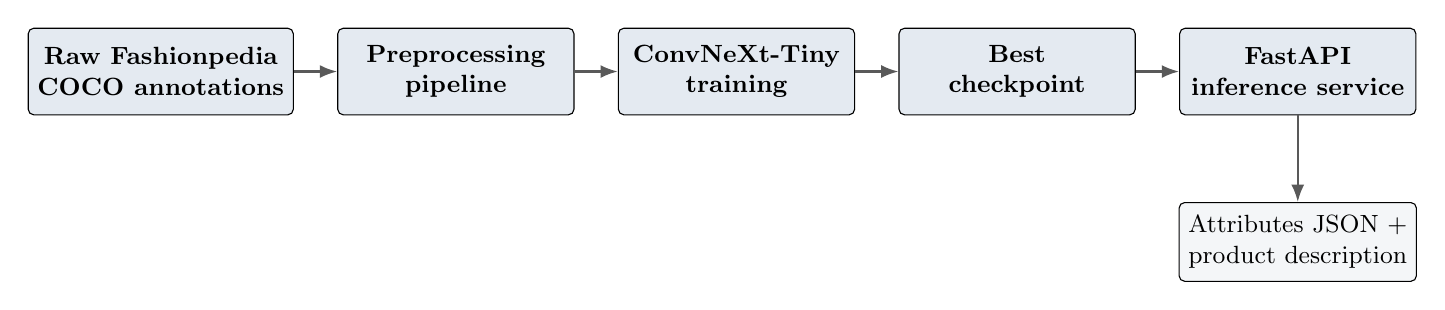
\begin{tikzpicture}[
  box/.style={draw, rounded corners=2pt, fill=lightbg, minimum height=1cm, minimum width=2.6cm, align=center, font=\small},
  stage/.style={draw, rounded corners=2pt, fill=cobalt!12, minimum height=1.1cm, minimum width=3.0cm, align=center, font=\small\bfseries},
  arr/.style={-{Latex[length=2.2mm]}, thick, color=gray!70!black},
  node distance=0.55cm
]
\node[stage] (raw) {Raw Fashionpedia\\ COCO annotations};
\node[stage, right=of raw] (prep) {Preprocessing\\ pipeline};
\node[stage, right=of prep] (train) {ConvNeXt-Tiny\\ training};
\node[stage, right=of train] (ckpt) {Best\\ checkpoint};
\node[stage, right=of ckpt] (api) {FastAPI\\ inference service};

\draw[arr] (raw) -- (prep);
\draw[arr] (prep) -- (train);
\draw[arr] (train) -- (ckpt);
\draw[arr] (ckpt) -- (api);

\node[box, below=1.1cm of api, minimum width=3.0cm] (out) {Attributes JSON +\\ product description};
\draw[arr] (api) -- (out);
\end{tikzpicture}
\caption{Top-level project flow: dataset $\to$ preprocessing $\to$ training $\to$ checkpoint $\to$ serving.}
\label{fig:system-overview}
\end{figure}

% =====================================================================
\section{Dataset: Fashionpedia}
% =====================================================================

\subsection{Source and raw statistics}

Fashionpedia annotates fashion product images at two levels: garment-part \textbf{instance segmentation} (46 categories, e.g. \emph{sleeve}, \emph{dress}, \emph{neckline}) and per-instance \textbf{visual attributes} (294 fine-grained attribute labels grouped into supercategories such as \emph{silhouette}, \emph{length}, \emph{textile pattern}). The project uses the \code{instances\_attributes\_train2020.json} / \code{instances\_attributes\_val2020.json} files.

\begin{table}[h]
\centering
\begin{tabular}{lrr}
\toprule
\textbf{Metric} & \textbf{Train} & \textbf{Val} \\
\midrule
Total annotations & 333{,}401 & 8{,}781 \\
Total images & 45{,}623 & 1{,}158 \\
Annotations with $\geq 1$ attribute & 206{,}410 (61.9\%) & 5{,}259 (59.9\%) \\
Mean attributes / annotation (raw) & 2.28 & 2.36 \\
Total categories & 46 & 46 \\
Total attributes & 294 & 294 \\
\bottomrule
\end{tabular}
\caption{Raw Fashionpedia statistics before preprocessing.}
\end{table}

\subsection{Preprocessing pipeline and design rationale}

The pipeline (\code{fashionpedia\_preprocessing.py}) is deliberately \emph{not} generic --- every step encodes a decision grounded in the dataset's specific pathologies:

\begin{enumerate}
\item \textbf{Drop zero-attribute annotations} (38.1\% of train). Fashionpedia annotators frequently skipped labeling attributes for an instance rather than confirming ``no attributes present.'' Treating skipped instances as confirmed all-negative rows would inject label noise into the BCE loss, so they are removed rather than kept as negatives.
\item \textbf{Exclude the \emph{nickname}, \emph{animal}, and \emph{leather} supercategories.} \emph{Nickname} attributes (e.g. ``jeans'', ``blazer'') are really garment-type identifiers that overlap with the category field and dominate the long tail; \emph{animal} and \emph{leather} have too few positive samples ($\leq$ 210) to be learnable under BCE.
\item \textbf{Rarity filter}: attributes with fewer than 300 training samples are dropped as unlearnable given the class-imbalance-aware loss still needs enough positives per batch to produce a gradient signal.
\item \textbf{Drop small/degenerate bounding boxes} (area $< 1024\,\text{px}^2$ or side $< 16\,\text{px}$) and duplicate crops.
\item \textbf{Train at the annotation (crop) level, not the full image}, since attributes describe individual garment parts, not the photo as a whole.
\item \textbf{Compute per-class \code{pos\_weight}} for \code{BCEWithLogitsLoss} from the cleaned label matrix, and build a category$\leftrightarrow$attribute-supercategory affinity table for optional soft/hard logit masking in future experiments.
\end{enumerate}

Figure~\ref{fig:preprocess-flow} diagrams the pipeline; Table~\ref{tab:cleaning} quantifies the impact of each cleaning step.

\begin{figure}[h]
\centering
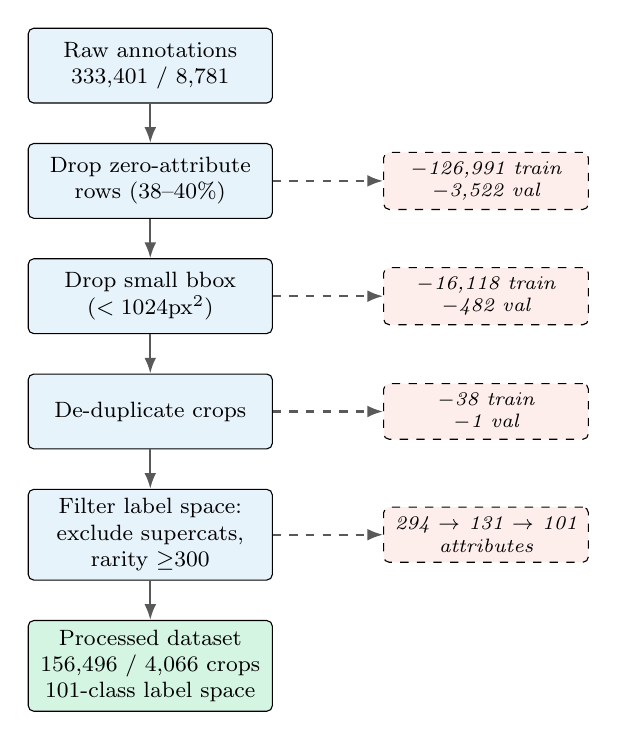
\begin{tikzpicture}[
  pstep/.style={draw, rounded corners=2pt, fill=accent2!12, minimum height=0.95cm, minimum width=3.1cm, align=center, font=\footnotesize},
  drop/.style={draw, rounded corners=2pt, fill=accent3!10, minimum height=0.7cm, minimum width=2.6cm, align=center, font=\scriptsize\itshape, dashed},
  arr/.style={-{Latex[length=2mm]}, thick, gray!70!black},
  node distance=0.5cm and 0.9cm
]
\node[pstep] (raw) {Raw annotations\\ 333{,}401 / 8{,}781};
\node[pstep, below=of raw] (zero) {Drop zero-attribute\\ rows (38--40\%)};
\node[pstep, below=of zero] (bbox) {Drop small bbox\\ ($<1024\text{px}^2$)};
\node[pstep, below=of bbox] (dup) {De-duplicate crops};
\node[pstep, below=of dup] (labelspace) {Filter label space:\\ exclude supercats,\\ rarity $\geq$300};
\node[pstep, below=of labelspace, fill=trainc!20] (final) {Processed dataset\\ 156{,}496 / 4{,}066 crops\\ 101-class label space};

\draw[arr] (raw) -- (zero);
\draw[arr] (zero) -- (bbox);
\draw[arr] (bbox) -- (dup);
\draw[arr] (dup) -- (labelspace);
\draw[arr] (labelspace) -- (final);

\node[drop, right=1.4cm of zero] (dzero) {$-$126{,}991 train\\ $-$3{,}522 val};
\node[drop, right=1.4cm of bbox] (dbbox) {$-$16{,}118 train\\ $-$482 val};
\node[drop, right=1.4cm of dup] (ddup) {$-$38 train\\ $-$1 val};
\node[drop, right=1.4cm of labelspace] (dlabel) {294 $\to$ 131 $\to$ 101\\ attributes};

\draw[arr, dashed] (zero.east) -- (dzero.west);
\draw[arr, dashed] (bbox.east) -- (dbbox.west);
\draw[arr, dashed] (dup.east) -- (ddup.west);
\draw[arr, dashed] (labelspace.east) -- (dlabel.west);
\end{tikzpicture}
\caption{Preprocessing pipeline: sequential cleaning steps and their effect on annotation count and label-space size.}
\label{fig:preprocess-flow}
\end{figure}

\begin{table}[h]
\centering
\small
\begin{tabular}{llrrrr}
\toprule
\textbf{Step} & \textbf{Split} & \textbf{Before} & \textbf{After} & \textbf{Removed} & \textbf{\% removed} \\
\midrule
drop\_zero\_attr   & train & 333{,}401 & 206{,}410 & 126{,}991 & 38.1\% \\
drop\_small\_bbox  & train & 206{,}410 & 190{,}292 & 16{,}118  & 7.8\%  \\
detect\_duplicates & train & 190{,}292 & 190{,}254 & 38        & 0.0\%  \\
\midrule
drop\_zero\_attr   & val   & 8{,}781   & 5{,}259   & 3{,}522   & 40.1\% \\
drop\_small\_bbox  & val   & 5{,}259   & 4{,}777   & 482       & 9.2\%  \\
detect\_duplicates & val   & 4{,}777   & 4{,}776   & 1         & 0.0\%  \\
\bottomrule
\end{tabular}
\caption{Impact of each cleaning step on annotation counts (\code{preprocessing\_report.md}).}
\label{tab:cleaning}
\end{table}

\subsection{Label space and class imbalance}

Of the original 294 attributes, excluding \emph{animal}, \emph{leather}, and \emph{nickname} leaves 131; applying the $\geq$300-sample rarity filter leaves \textbf{101 retained attributes} across 8 supercategories. Figure~\ref{fig:attr-dist} shows the long-tailed frequency distribution and which attributes were retained vs.\ dropped; Figure~\ref{fig:supercat} shows the final label space broken down by supercategory.

\begin{figure}[h]
\centering
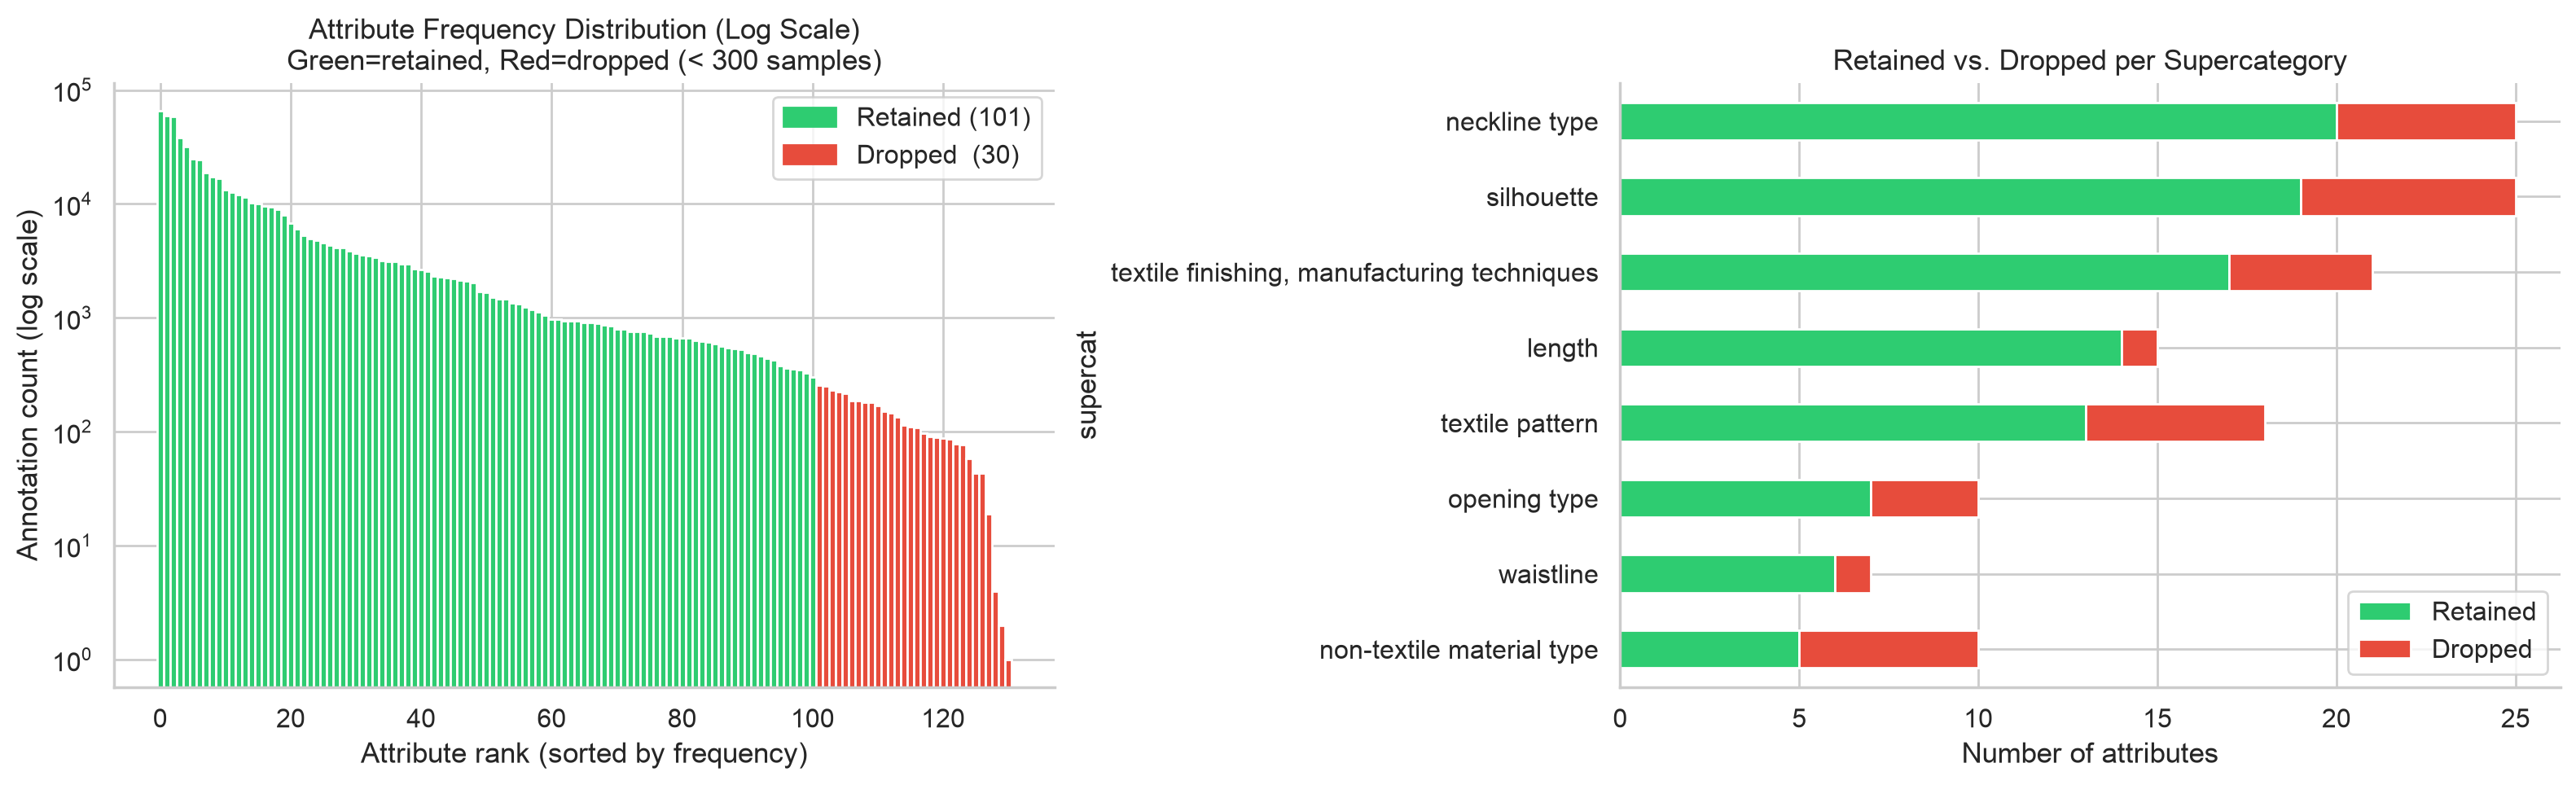
\includegraphics[width=\linewidth]{fig1_attribute_distribution.png}
\caption{Left: attribute frequency distribution (log scale), green = retained (101), red = dropped for rarity (30). Right: retained vs.\ dropped attribute counts per supercategory.}
\label{fig:attr-dist}
\end{figure}

\begin{figure}[h]
\centering
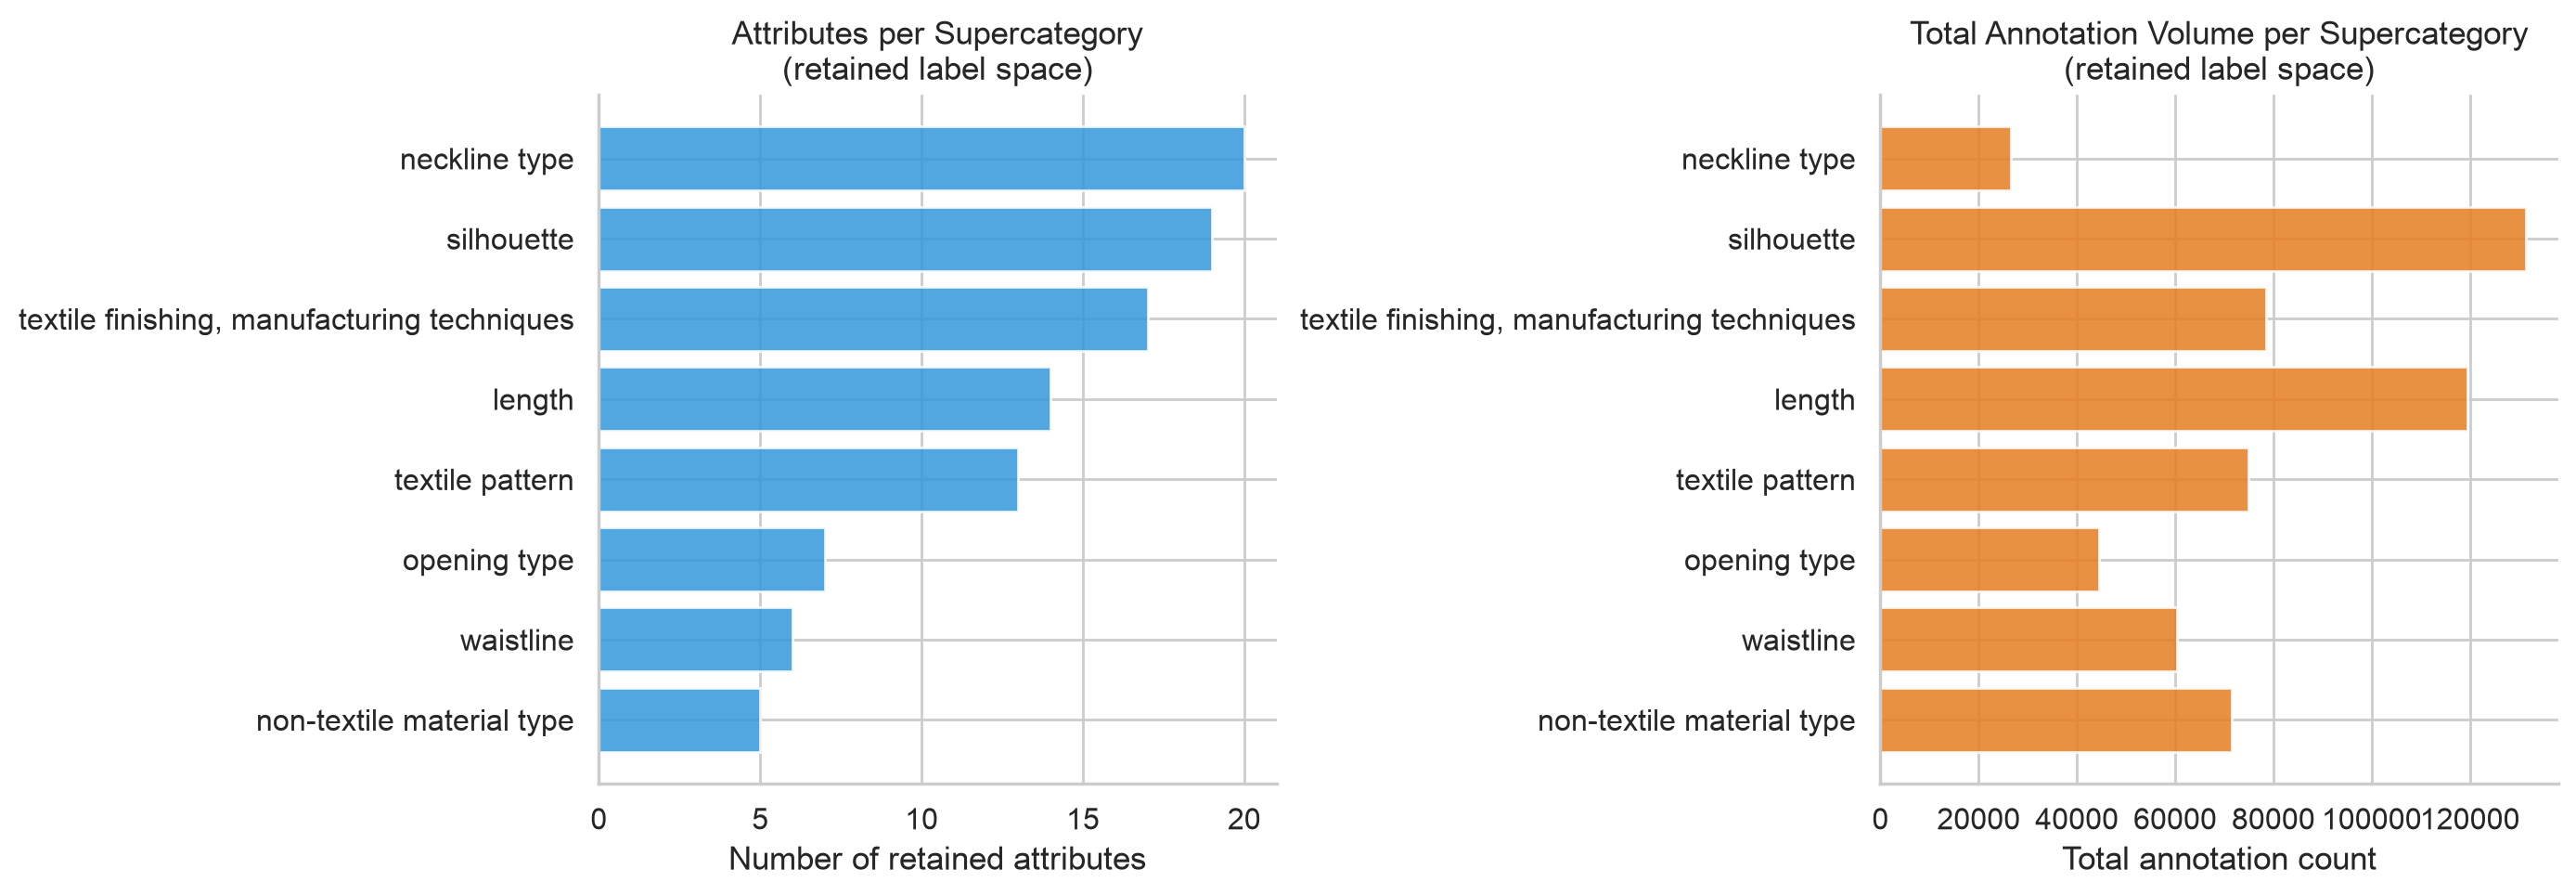
\includegraphics[width=\linewidth]{fig6_supercat_breakdown.png}
\caption{Final 101-attribute label space: number of attributes (left) and total annotation volume (right) per supercategory. \emph{Neckline type} contributes the most distinct attributes (20); \emph{silhouette} and \emph{length} contribute the most annotation volume.}
\label{fig:supercat}
\end{figure}

Even after filtering, the retained label space is heavily imbalanced: the BCE positive weight (negative/positive ratio) ranges from 1.38 to 515.5 across the 101 classes (median 92.5, mean 135.8). Figure~\ref{fig:imbalance} shows the distribution and the most imbalanced attributes; \code{paisley}, \code{queen anne (neck)}, and \code{lace up} are the hardest (rarest) positive classes.

\begin{figure}[h]
\centering
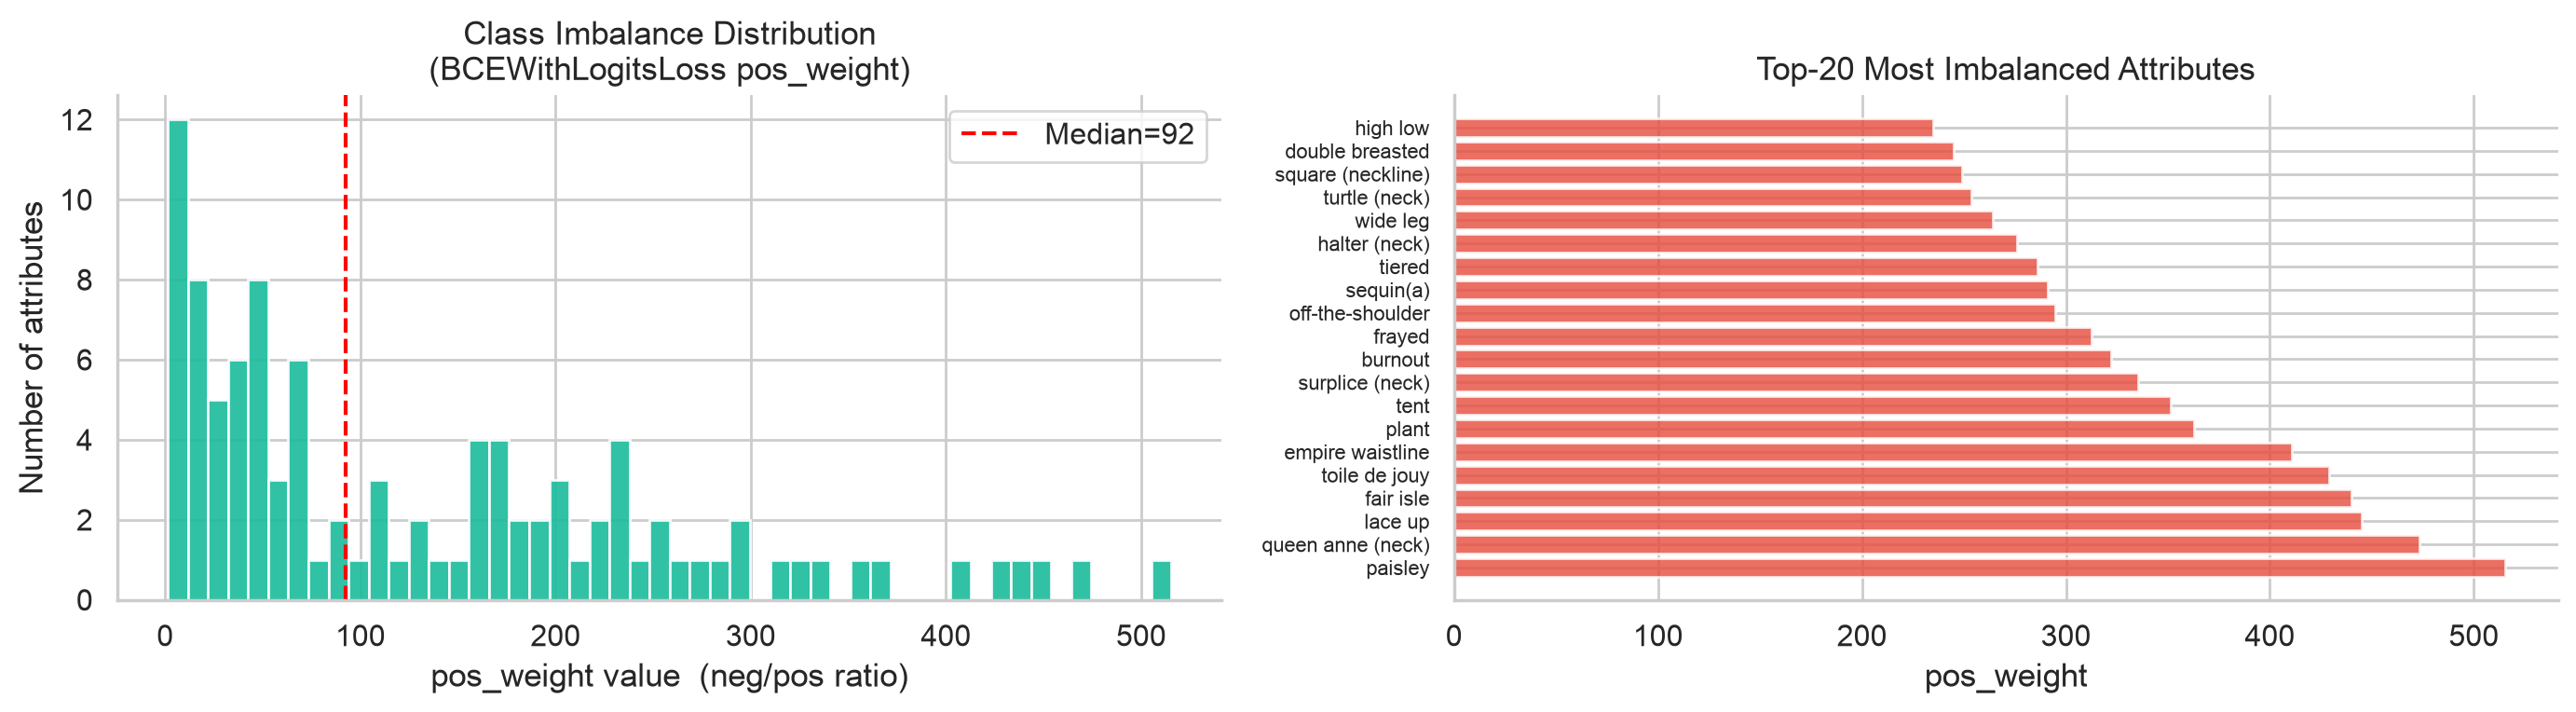
\includegraphics[width=\linewidth]{fig4_class_imbalance.png}
\caption{Left: histogram of per-class \code{pos\_weight} (median = 92, dashed line). Right: the 20 most imbalanced retained attributes.}
\label{fig:imbalance}
\end{figure}

\subsection{Processed dataset and image/category distribution}

The final processed dataset comprises \textbf{156{,}496 training crops} (45{,}589 unique images) and \textbf{4{,}066 validation crops} (1{,}158 unique images), each a garment-part bounding-box crop paired with a 101-dimensional multi-hot label vector. Figure~\ref{fig:cat-dist} shows that \emph{sleeve} dominates the category distribution by a wide margin, followed by \emph{neckline} and \emph{dress}. Figure~\ref{fig:attrs-per-ann} shows that despite a mean of 3.88 attributes per annotation, the \emph{median} is only 1 --- the distribution is bimodal, with a large single-attribute mode and a secondary mode around 7--9 attributes (multi-attribute garment parts like full dresses).

\begin{figure}[h]
\centering
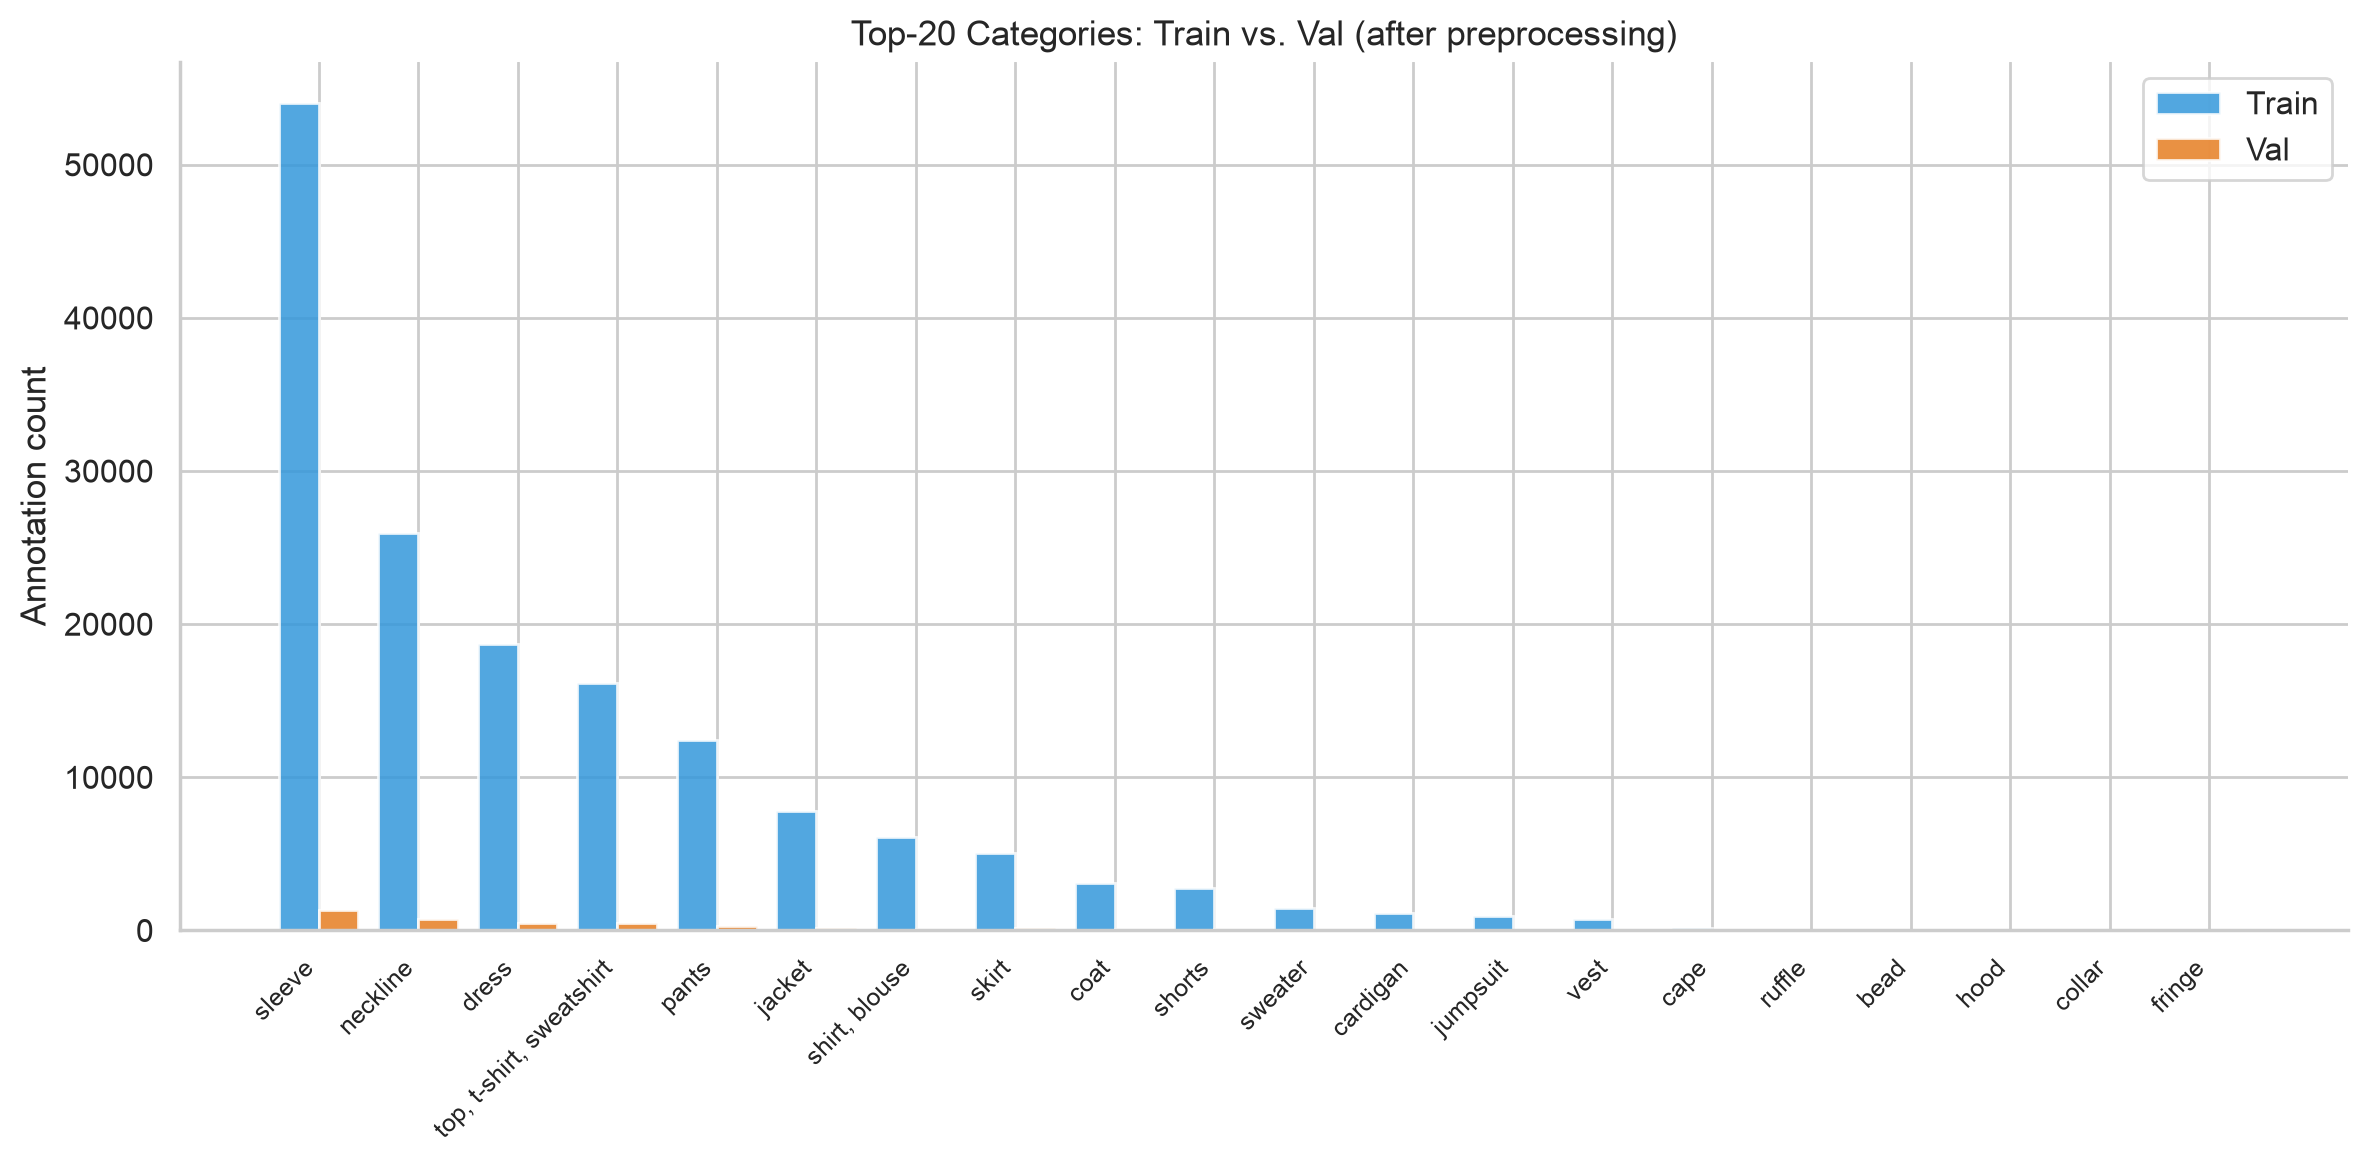
\includegraphics[width=0.85\linewidth]{fig2_category_distribution.png}
\caption{Top-20 garment-part categories after preprocessing, train vs.\ val.}
\label{fig:cat-dist}
\end{figure}

\begin{figure}[h]
\centering
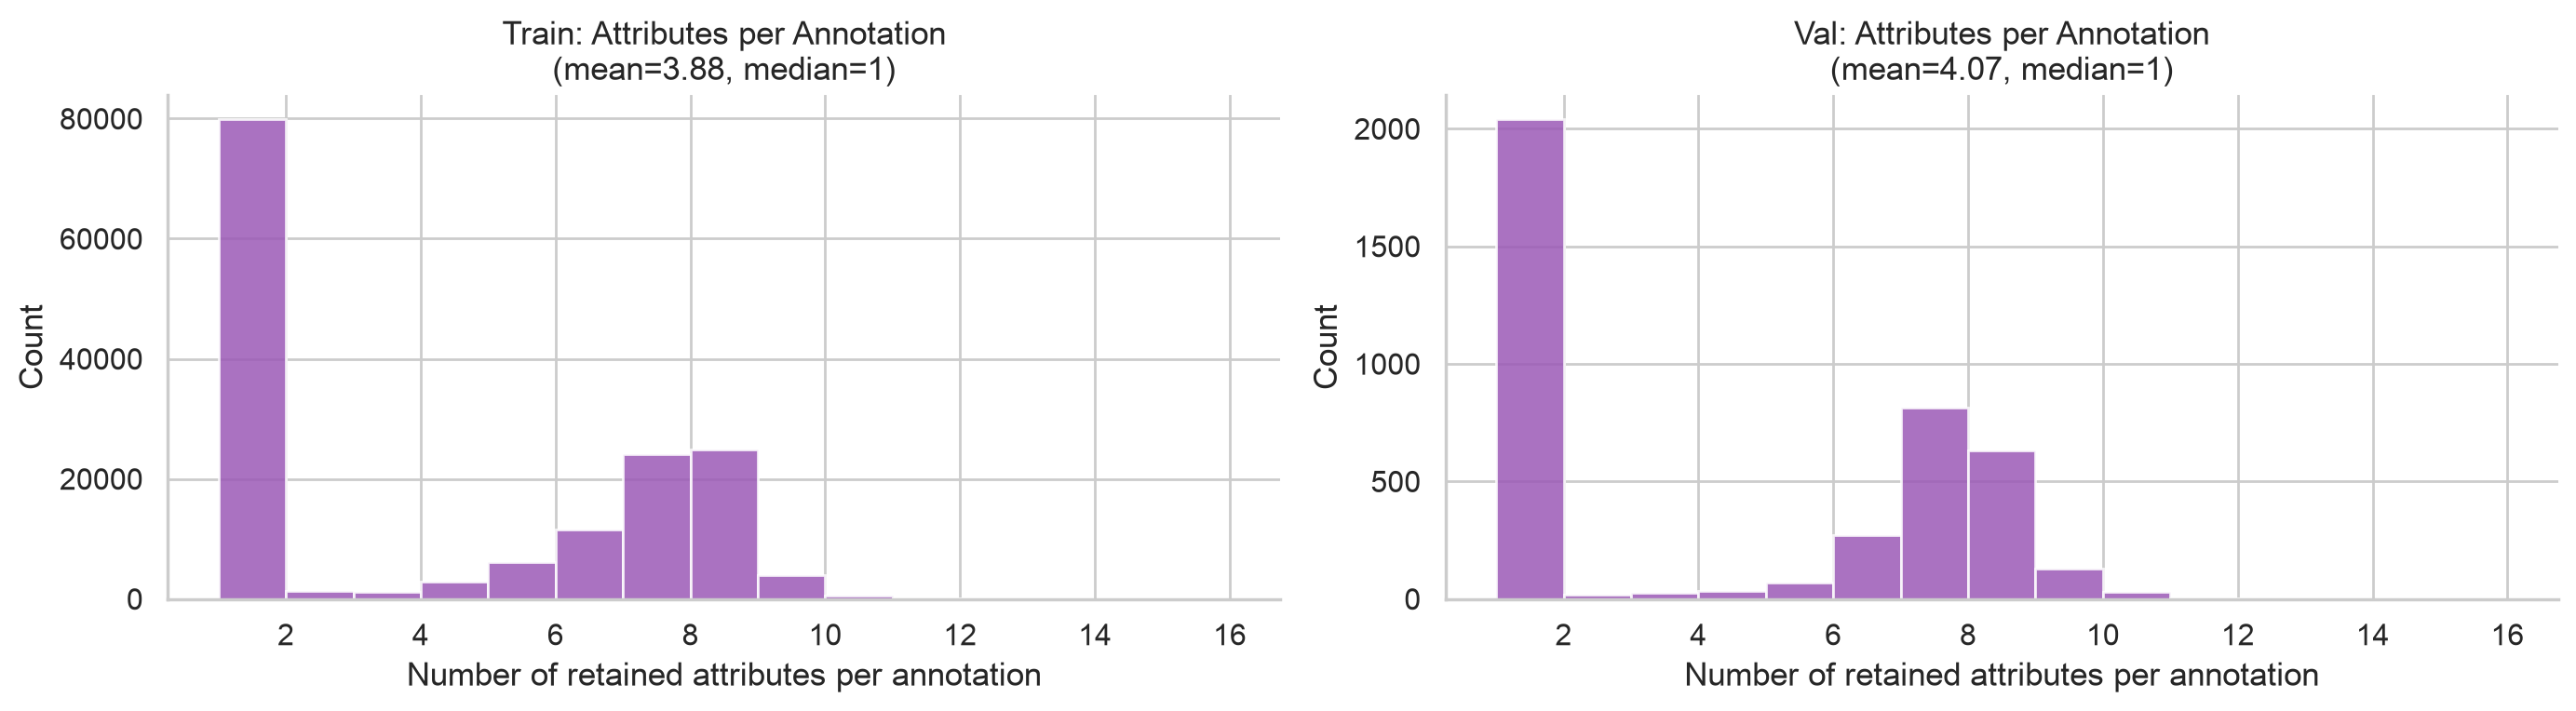
\includegraphics[width=\linewidth]{fig3_attrs_per_annotation.png}
\caption{Distribution of number of retained attributes per annotation, train (left) and val (right).}
\label{fig:attrs-per-ann}
\end{figure}

Quality-assurance checks reported zero all-zero label vectors, zero duplicate crops, zero train/val image leakage, and zero missing image files in either split. A category$\leftrightarrow$attribute-supercategory affinity table (Figure~\ref{fig:affinity}) was also computed for possible use as a soft prior or hard logit mask; in the exported artifact all cells evaluate to 0.00, which reflects a normalization convention in the affinity computation rather than genuine independence between categories and attributes, and is flagged here as a known rough edge in the preprocessing pipeline rather than a modeling result. This affinity mask was \emph{not} applied during training (\code{apply\_category\_attr\_masking = False}).

\begin{figure}[h]
\centering
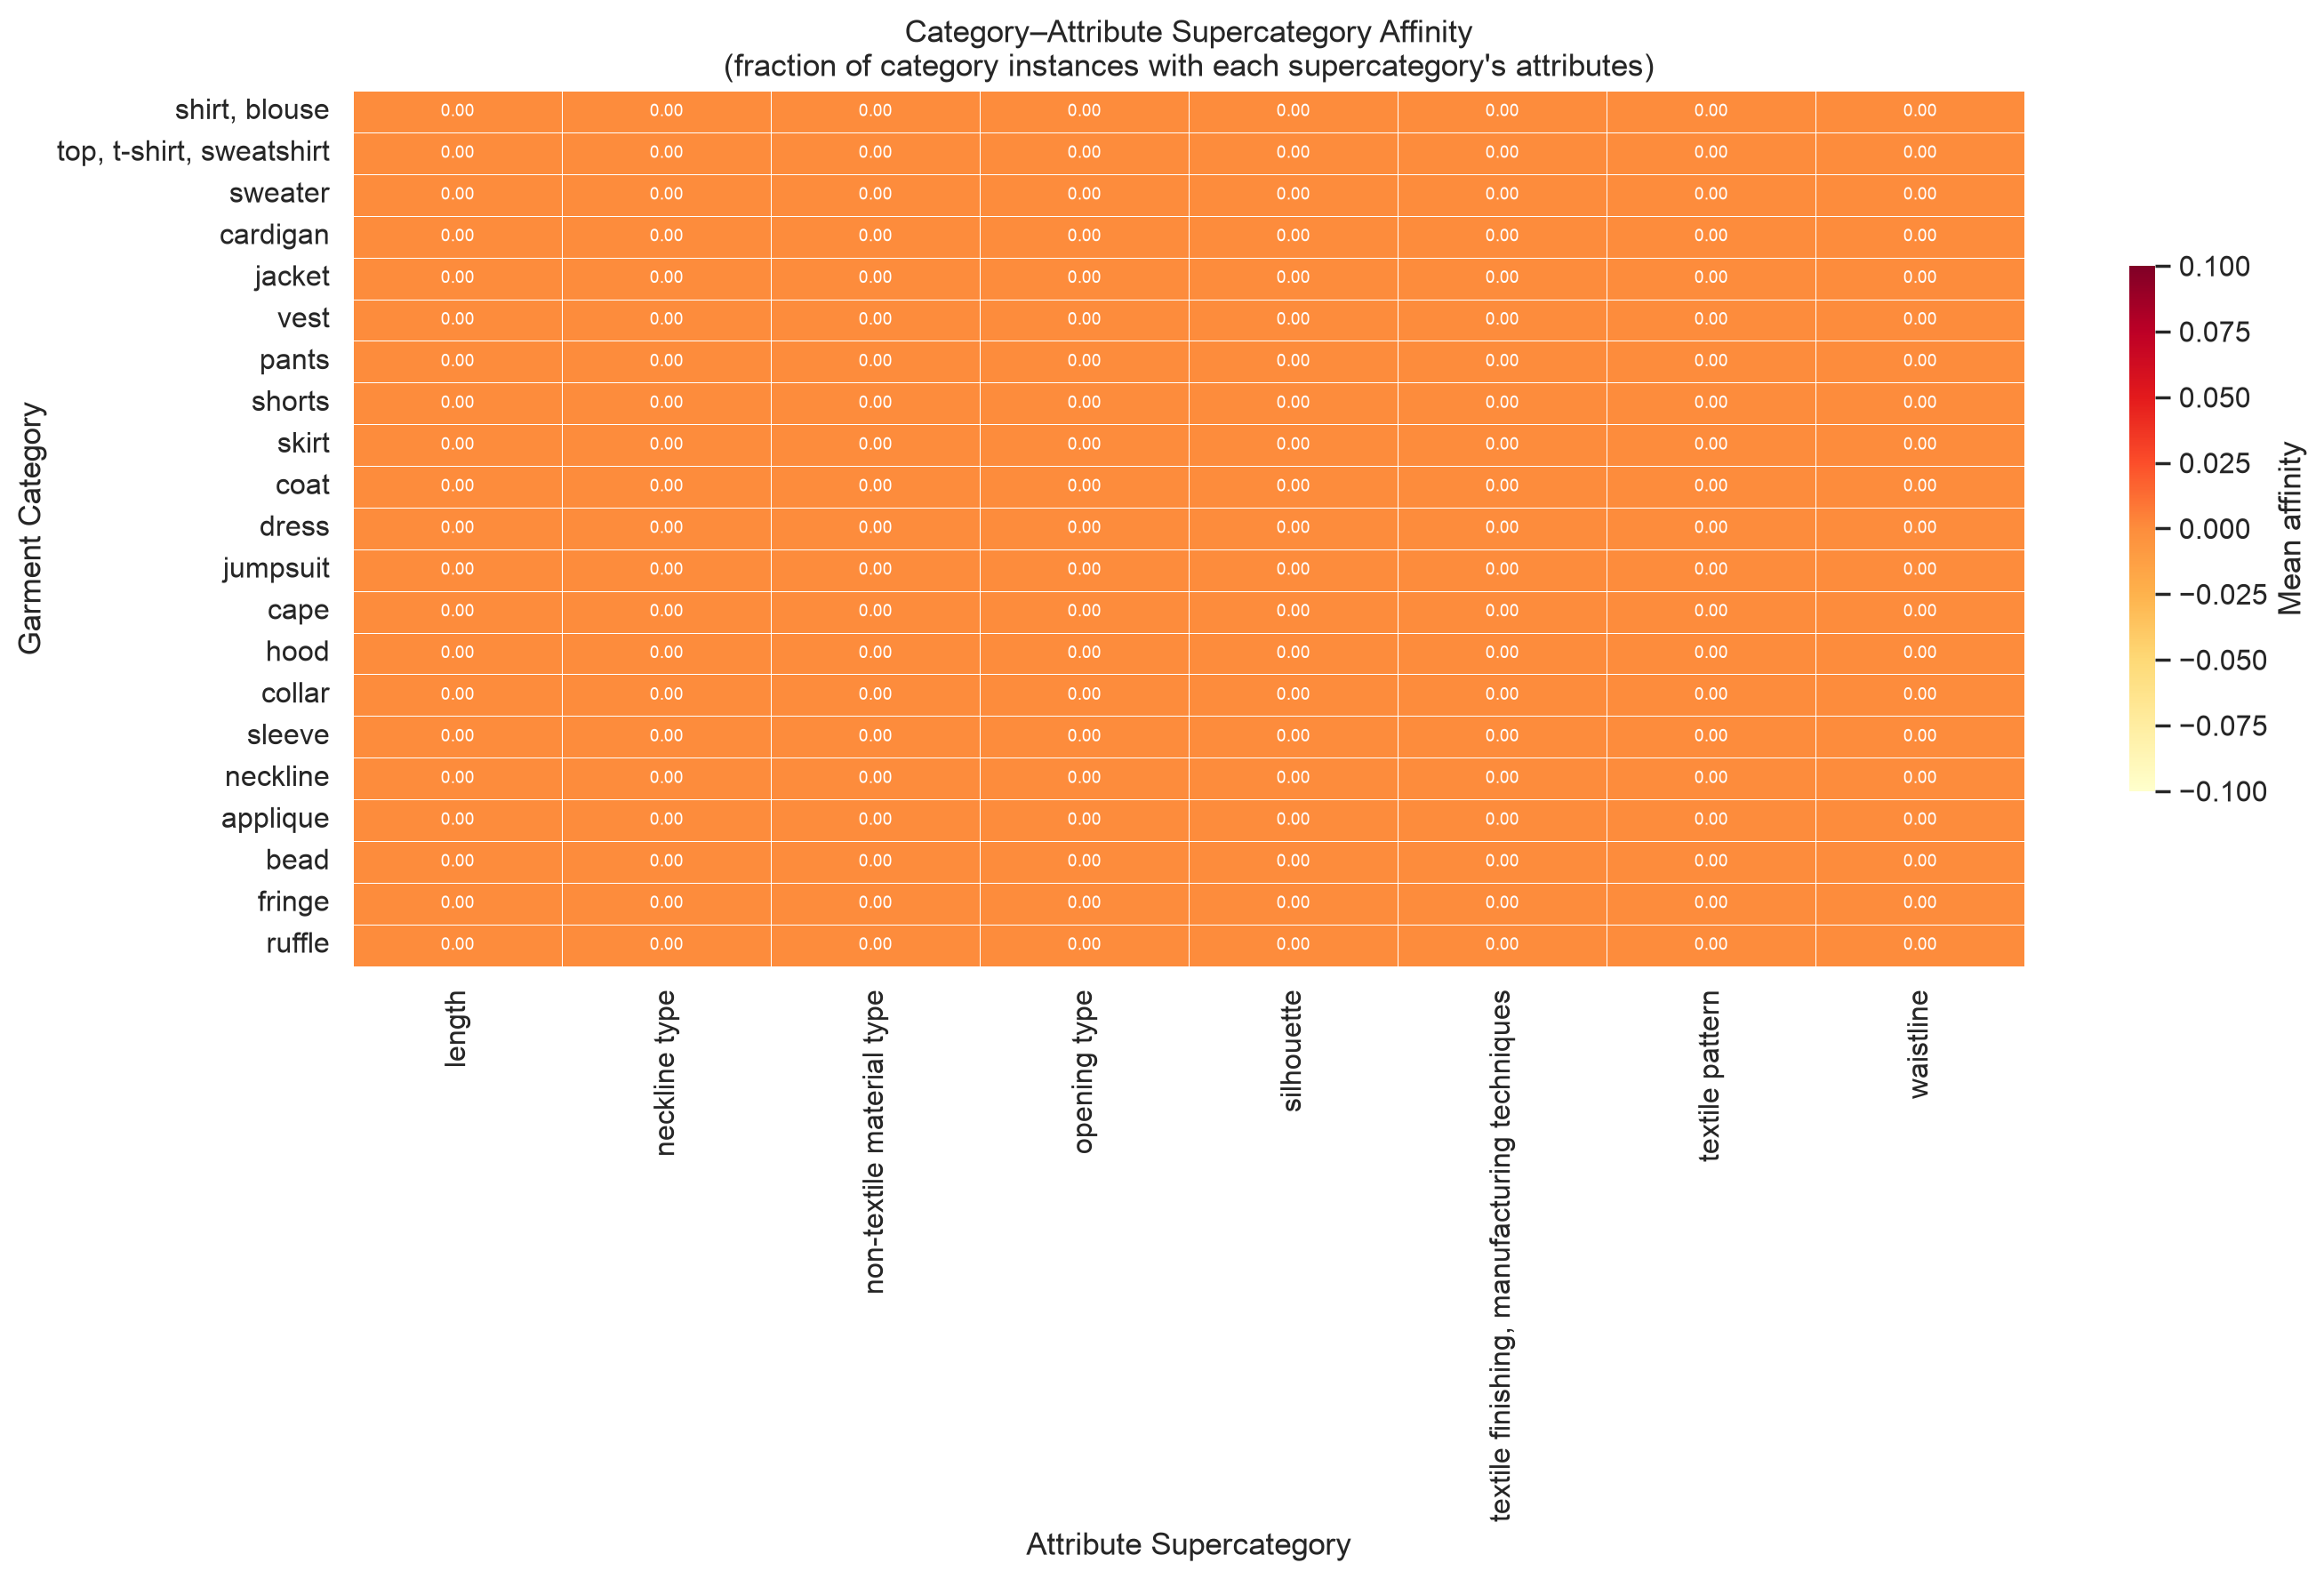
\includegraphics[width=0.9\linewidth]{fig5_affinity_heatmap.png}
\caption{Category$\times$attribute-supercategory affinity heatmap, as exported by the preprocessing pipeline. All cells read 0.00 in this artifact --- see caveat above.}
\label{fig:affinity}
\end{figure}

\begin{table}[h]
\centering
\begin{tabular}{lrr}
\toprule
\textbf{Metric} & \textbf{Train} & \textbf{Val} \\
\midrule
Annotations (crops) & 156{,}496 & 4{,}066 \\
Unique images & 45{,}589 & 1{,}158 \\
Label space size & 101 & 101 \\
Mean attrs / annotation & 3.88 & 4.07 \\
Median attrs / annotation & 1 & 1 \\
Annotations with a negation attribute & 70{,}613 (45.1\%) & 1{,}900 (46.7\%) \\
\bottomrule
\end{tabular}
\caption{Final processed dataset statistics.}
\end{table}

% =====================================================================
\section{Model Architecture}
% =====================================================================

\subsection{Backbone and head}

The classifier is a \textbf{ConvNeXt-Tiny} (ImageNet-1K-pretrained, $\sim$28M parameters) with its original 1000-way ImageNet head removed, followed by a custom 2-layer MLP head for 101-way multi-label prediction. ConvNeXt-Tiny's \code{features} module is a sequential stack of 8 blocks: a stem, four stage blocks, and three downsampling layers interleaved between them (indices 0--7, with index 7 = the deepest / most task-specific stage). The output after adaptive average pooling is a 768-dimensional feature vector.

\begin{center}
\begin{tabular}{ll}
\toprule
\textbf{Head component} & \textbf{Shape / operation} \\
\midrule
\code{LayerNorm} & (768) --- stabilizes pooled features \\
\code{Linear} & 768 $\to$ 512 \\
\code{GELU} & activation (matches ConvNeXt's own nonlinearity) \\
\code{Dropout} & $p=0.3$ \\
\code{Linear} & 512 $\to$ 101 (raw logits, no sigmoid) \\
\bottomrule
\end{tabular}
\end{center}

The head is a 2-layer MLP rather than a single linear layer because a nonlinear projection lets the model re-compose ImageNet-pretrained visual features into fashion-domain attribute combinations, and dropout regularizes the (randomly initialized, higher-LR) head independently of the backbone's weight decay.

\subsection{Partial fine-tuning and the ablation axis}

Training uses a single knob, \code{unfreeze\_from\_block}, to control how much of the backbone is trainable: everything in \code{features[0:unfreeze\_from\_block]} is frozen (including its LayerNorm parameters --- correct for ConvNeXt, which uses LayerNorm rather than BatchNorm), and \code{features[unfreeze\_from\_block:8]} plus the head remain trainable. Three configurations were prepared as an ablation study (Table~\ref{tab:ablation-configs}); only \textbf{Ablation B} was actually trained to a meaningful number of epochs in this repository (see Section~\ref{sec:results}).

\begin{table}[h]
\centering
\begin{tabular}{lccccl}
\toprule
\textbf{Config} & \textbf{unfreeze\_from} & \textbf{lr\_backbone} & \textbf{Epochs} & \textbf{Warmup} & \textbf{Role} \\
\midrule
A --- head only     & 8 & 0 (frozen)      & 20 & 3 & Lower-bound baseline \\
\rowcolor{cobalt!8} B --- stage-4 + head & 6 & $1\times10^{-4}$ & 30 & 3 & \textbf{Default / recommended} \\
C --- stages 3--4 + head & 4 & $5\times10^{-5}$ & 30 & 5 & More capacity, used if B plateaus \\
\bottomrule
\end{tabular}
\caption{Ablation configurations over how much of the ConvNeXt-Tiny backbone is unfrozen.}
\label{tab:ablation-configs}
\end{table}

Figure~\ref{fig:model-arch} illustrates the backbone/head architecture and which blocks are frozen vs.\ trainable under the Ablation-B configuration actually used for the reported run.

\begin{figure}[h]
\centering
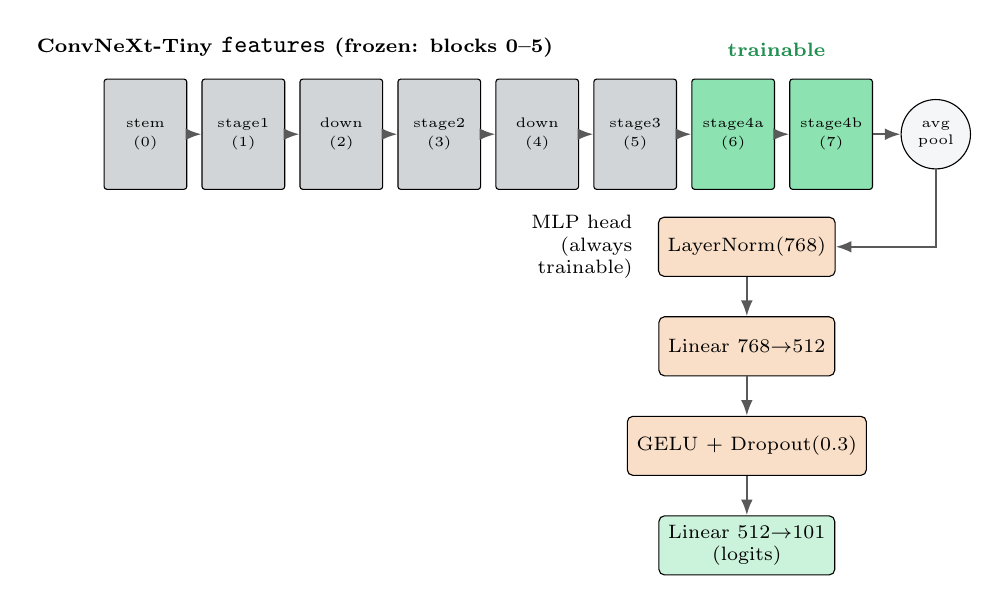
\begin{tikzpicture}[
  blk/.style={draw, rounded corners=1pt, minimum width=1.05cm, minimum height=1.4cm, align=center, font=\tiny},
  hd/.style={draw, rounded corners=2pt, fill=headc!25, minimum width=2.1cm, minimum height=0.75cm, align=center, font=\scriptsize},
  arr/.style={-{Latex[length=2mm]}, thick, gray!70!black},
  node distance=0.18cm
]
% Feature blocks 0..7
\node[blk, fill=frozenc!70] (b0) {stem\\[1pt](0)};
\node[blk, fill=frozenc!70, right=of b0] (b1) {stage1\\[1pt](1)};
\node[blk, fill=frozenc!70, right=of b1] (b2) {down\\[1pt](2)};
\node[blk, fill=frozenc!70, right=of b2] (b3) {stage2\\[1pt](3)};
\node[blk, fill=frozenc!70, right=of b3] (b4) {down\\[1pt](4)};
\node[blk, fill=frozenc!70, right=of b4] (b5) {stage3\\[1pt](5)};
\node[blk, fill=trainc!55, right=of b5] (b6) {stage4a\\[1pt](6)};
\node[blk, fill=trainc!55, right=of b6] (b7) {stage4b\\[1pt](7)};

\node[font=\scriptsize, above=0.15cm of b0, xshift=1.9cm] {\textbf{ConvNeXt-Tiny \code{features} (frozen: blocks 0--5)}};
\node[font=\scriptsize, above=0.15cm of b6, xshift=0.55cm, text=trainc!70!black] {\textbf{trainable}};

\node[draw, circle, minimum size=0.55cm, right=0.35cm of b7, fill=lightbg, font=\tiny, align=center] (pool) {avg\\pool};
\draw[arr] (b0)--(b1); \draw[arr] (b1)--(b2); \draw[arr] (b2)--(b3);
\draw[arr] (b3)--(b4); \draw[arr] (b4)--(b5); \draw[arr] (b5)--(b6);
\draw[arr] (b6)--(b7); \draw[arr] (b7)--(pool);

\node[hd, below=0.6cm of pool, xshift=-2.4cm] (ln) {LayerNorm(768)};
\node[hd, below=0.5cm of ln] (l1) {Linear 768$\to$512};
\node[hd, below=0.5cm of l1] (gelu) {GELU + Dropout(0.3)};
\node[hd, below=0.5cm of gelu, fill=accent1!25] (l2) {Linear 512$\to$101\\ (logits)};

\draw[arr] (pool) |- (ln);
\draw[arr] (ln) -- (l1);
\draw[arr] (l1) -- (gelu);
\draw[arr] (gelu) -- (l2);

\node[font=\scriptsize, left=0.2cm of ln, text width=1.6cm, align=right] {MLP head\\(always\\ trainable)};
\end{tikzpicture}
\caption{Model architecture under the Ablation-B configuration: ConvNeXt-Tiny blocks 0--5 frozen (grey), blocks 6--7 (``stage 4'') unfrozen (green), followed by the always-trainable MLP head.}
\label{fig:model-arch}
\end{figure}

\subsection{Loss function}

Multi-label prediction uses \code{BCEWithLogitsLoss} with a per-class \code{pos\_weight} tensor computed as $\text{pos\_weight}_i = n_{\text{neg},i} / n_{\text{pos},i}$ from the training split, capped at 50 (\code{pos\_weight\_cap}) to avoid numerically unstable gradients on the rarest classes. Without this weighting, gradient descent on BCE is dominated by the easy majority-negative signal and the model collapses to near-always-predicting-zero for rare attributes.

\subsection{Optimizer and learning-rate schedule}

AdamW is used with \textbf{differential learning rates}: $\text{lr}_{\text{head}} = 1\times10^{-3}$ for the randomly-initialized head, and $\text{lr}_{\text{backbone}} = 1\times10^{-4}$ (10$\times$ smaller) for the unfrozen backbone blocks, on the reasoning that pretrained weights should move slowly while the new head adapts quickly. Weight decay ($10^{-4}$) is applied only to weight matrices, not to biases or LayerNorm parameters. A 3-epoch linear warmup precedes a cosine-annealing schedule (Figure~\ref{fig:lr-schedule}) to prevent the initially-random head from destabilizing pretrained backbone features. Gradient norms are clipped to 1.0.

% =====================================================================
\section{Training Methodology}
% =====================================================================

\subsection{Data pipeline and augmentation}

Each training sample is a bounding-box crop resized to $224\times224$ (ConvNeXt-Tiny's native input size), normalized with ImageNet statistics. Training augmentation is deliberately curated for fashion imagery:

\begin{center}
\begin{tabular}{ll}
\toprule
\textbf{Used} & \textbf{Rationale} \\
\midrule
\code{RandomResizedCrop} (scale 0.7--1.0) & simulates zoom/framing variation \\
\code{RandomHorizontalFlip} ($p{=}0.5$) & garments are left-right symmetric \\
\code{RandomRotation} ($\pm10^{\circ}$) & small rotational invariance \\
\code{ColorJitter} (mild, hue $\leq 0.05$) & lighting variation without corrupting pattern/color attributes \\
\midrule
\textbf{Deliberately avoided} & \textbf{Rationale} \\
\midrule
Vertical flip & upside-down garments are semantically meaningless \\
Aggressive color distortion & would destroy texture/pattern attributes (stripe, floral, check) \\
Cutout / random erasing & can hide the exact region that carries the attribute signal \\
\bottomrule
\end{tabular}
\end{center}

Validation uses a deterministic resize-then-center-crop transform with no augmentation.

\subsection{Metrics}

Each epoch reports four validation metrics computed on sigmoid outputs: \textbf{mAP} (macro-averaged, threshold-free average precision --- the primary model-selection metric), and \textbf{macro F1 / Precision / Recall} at a fixed decision threshold (0.5 by default). A final threshold sweep (0.3/0.4/0.5/0.6) is intended to characterize the precision--recall trade-off of the best checkpoint.

\subsection{Runs actually executed}

Three run directories exist under \code{fashionpedia\_runs/}:

\begin{itemize}
\item \textbf{\code{run\_20260618\_040337}} and \textbf{\code{run\_20260618\_040727}} --- 2-epoch \emph{debug} sanity runs (\code{debug\_batches=2}), used to smoke-test the training loop, not meaningful models.
\item \textbf{\code{ablation\_B\_stage4\_head}} --- the substantive run, using the Ablation-B configuration (Table~\ref{tab:ablation-configs}): batch size 64, MPS device, 30 planned epochs.
\end{itemize}

Ablations A and C were configured (\code{config\_ablation\_A\_head\_only.json}, \code{config\_ablation\_C\_stages34\_head.json}) but \textbf{no corresponding run directories exist} --- they were not executed in this repository, so no A/B/C comparison is currently available.

% =====================================================================
\section{Results}
\label{sec:results}
% =====================================================================

\subsection{Training run status}

The Ablation-B run logged only \textbf{7 of the planned 30 epochs} (training log has 7 rows; only one periodic checkpoint, \code{epoch\_005.pt}, plus \code{best.pt}/\code{last.pt}, both from epoch 7). At roughly 24--26 minutes/epoch on MPS, this represents about 2.5 hours of training before the run stopped --- there is no evidence of an early-stopping trigger in the code (none is implemented), so the run was most likely interrupted manually or by the environment rather than converging. \textbf{Because \code{val\_mAP} was still rising at epoch 7}, \code{best.pt} and \code{last.pt} are identical, and the results below should be read as an \emph{early snapshot}, not a converged model. No final threshold sweep exists for this run (\code{threshold\_sweep.csv} is only present for the 2-epoch debug run and is not representative).

\begin{table}[h]
\centering
\begin{tabular}{lrrrr}
\toprule
\textbf{Epoch} & \textbf{Train loss} & \textbf{Val loss} & \textbf{Val mAP} & \textbf{Val F1 / P / R} \\
\midrule
1 & 0.432 & 0.461 & 0.319 & 0.258 / 0.179 / 0.747 \\
3 & 0.338 & 0.451 & 0.344 & 0.278 / 0.193 / 0.758 \\
5 & 0.309 & 0.451 & 0.355 & 0.282 / 0.194 / 0.775 \\
\rowcolor{cobalt!8} 7 (best) & 0.278 & 0.471 & \textbf{0.362} & 0.291 / 0.202 / 0.746 \\
\bottomrule
\end{tabular}
\caption{Selected epochs from the Ablation-B training log (\code{fashionpedia\_runs/ablation\_B\_stage4\_head/training\_log.csv}).}
\label{tab:results-table}
\end{table}

\subsection{Loss and metric curves}

\begin{figure}[h]
\centering
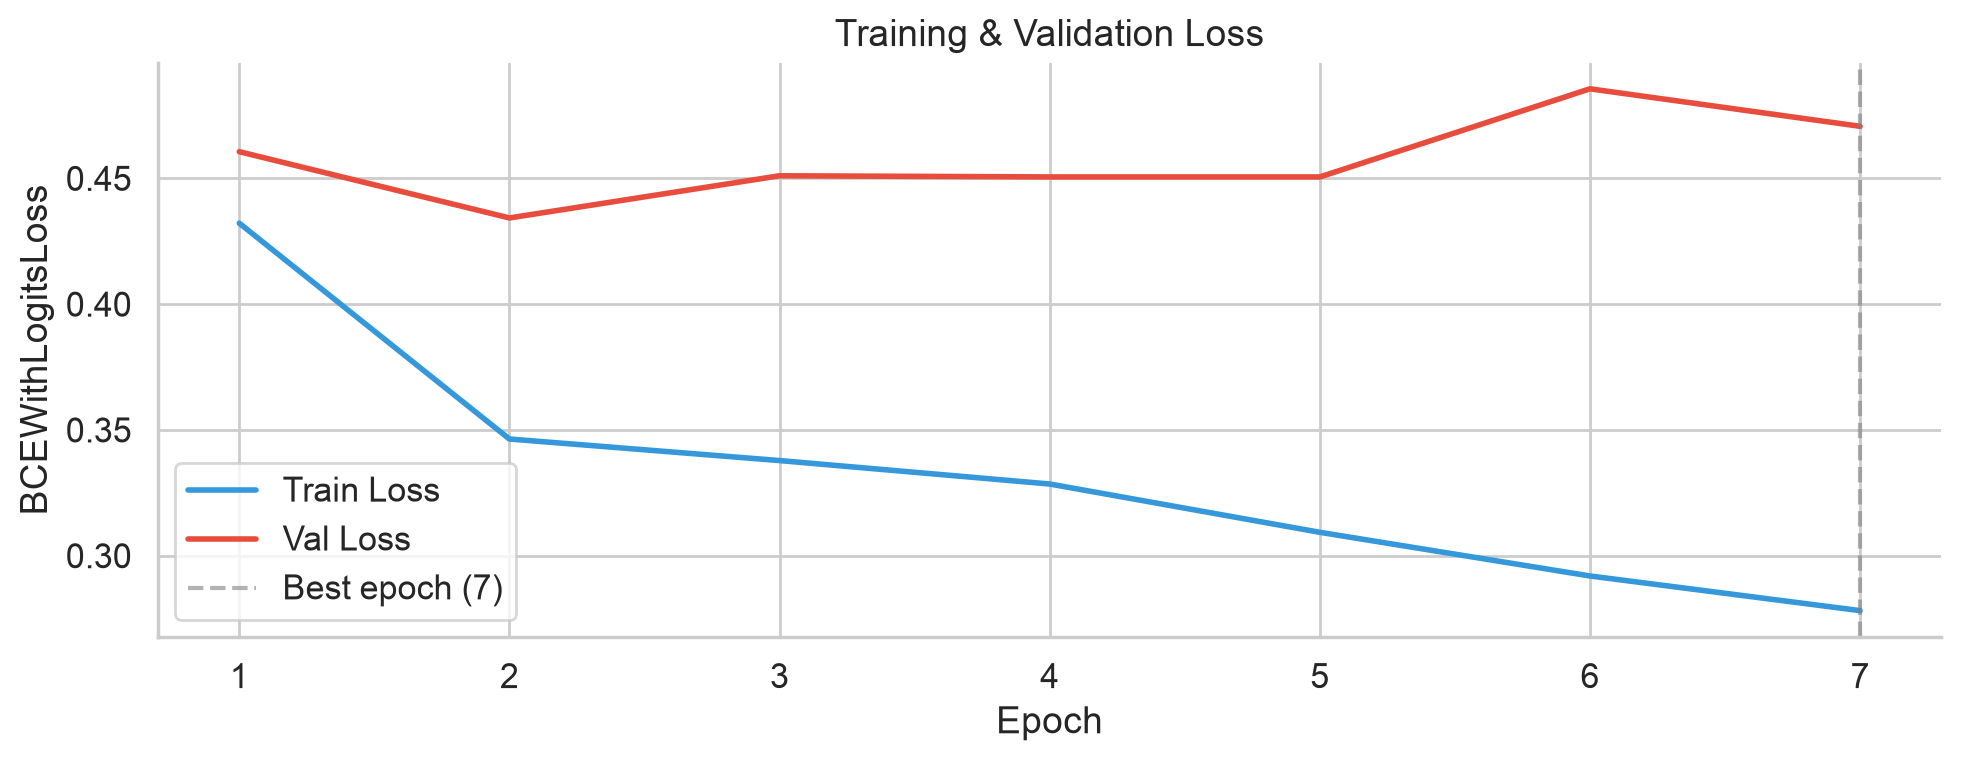
\includegraphics[width=0.85\linewidth]{loss_curves.png}
\caption{Train vs.\ validation BCE loss over the 7 completed epochs. Validation loss stops improving after epoch 2 and drifts upward from epoch 5 onward, while training loss keeps falling --- an early overfitting signal even though the run is short.}
\label{fig:loss-curves}
\end{figure}

\begin{figure}[h]
\centering
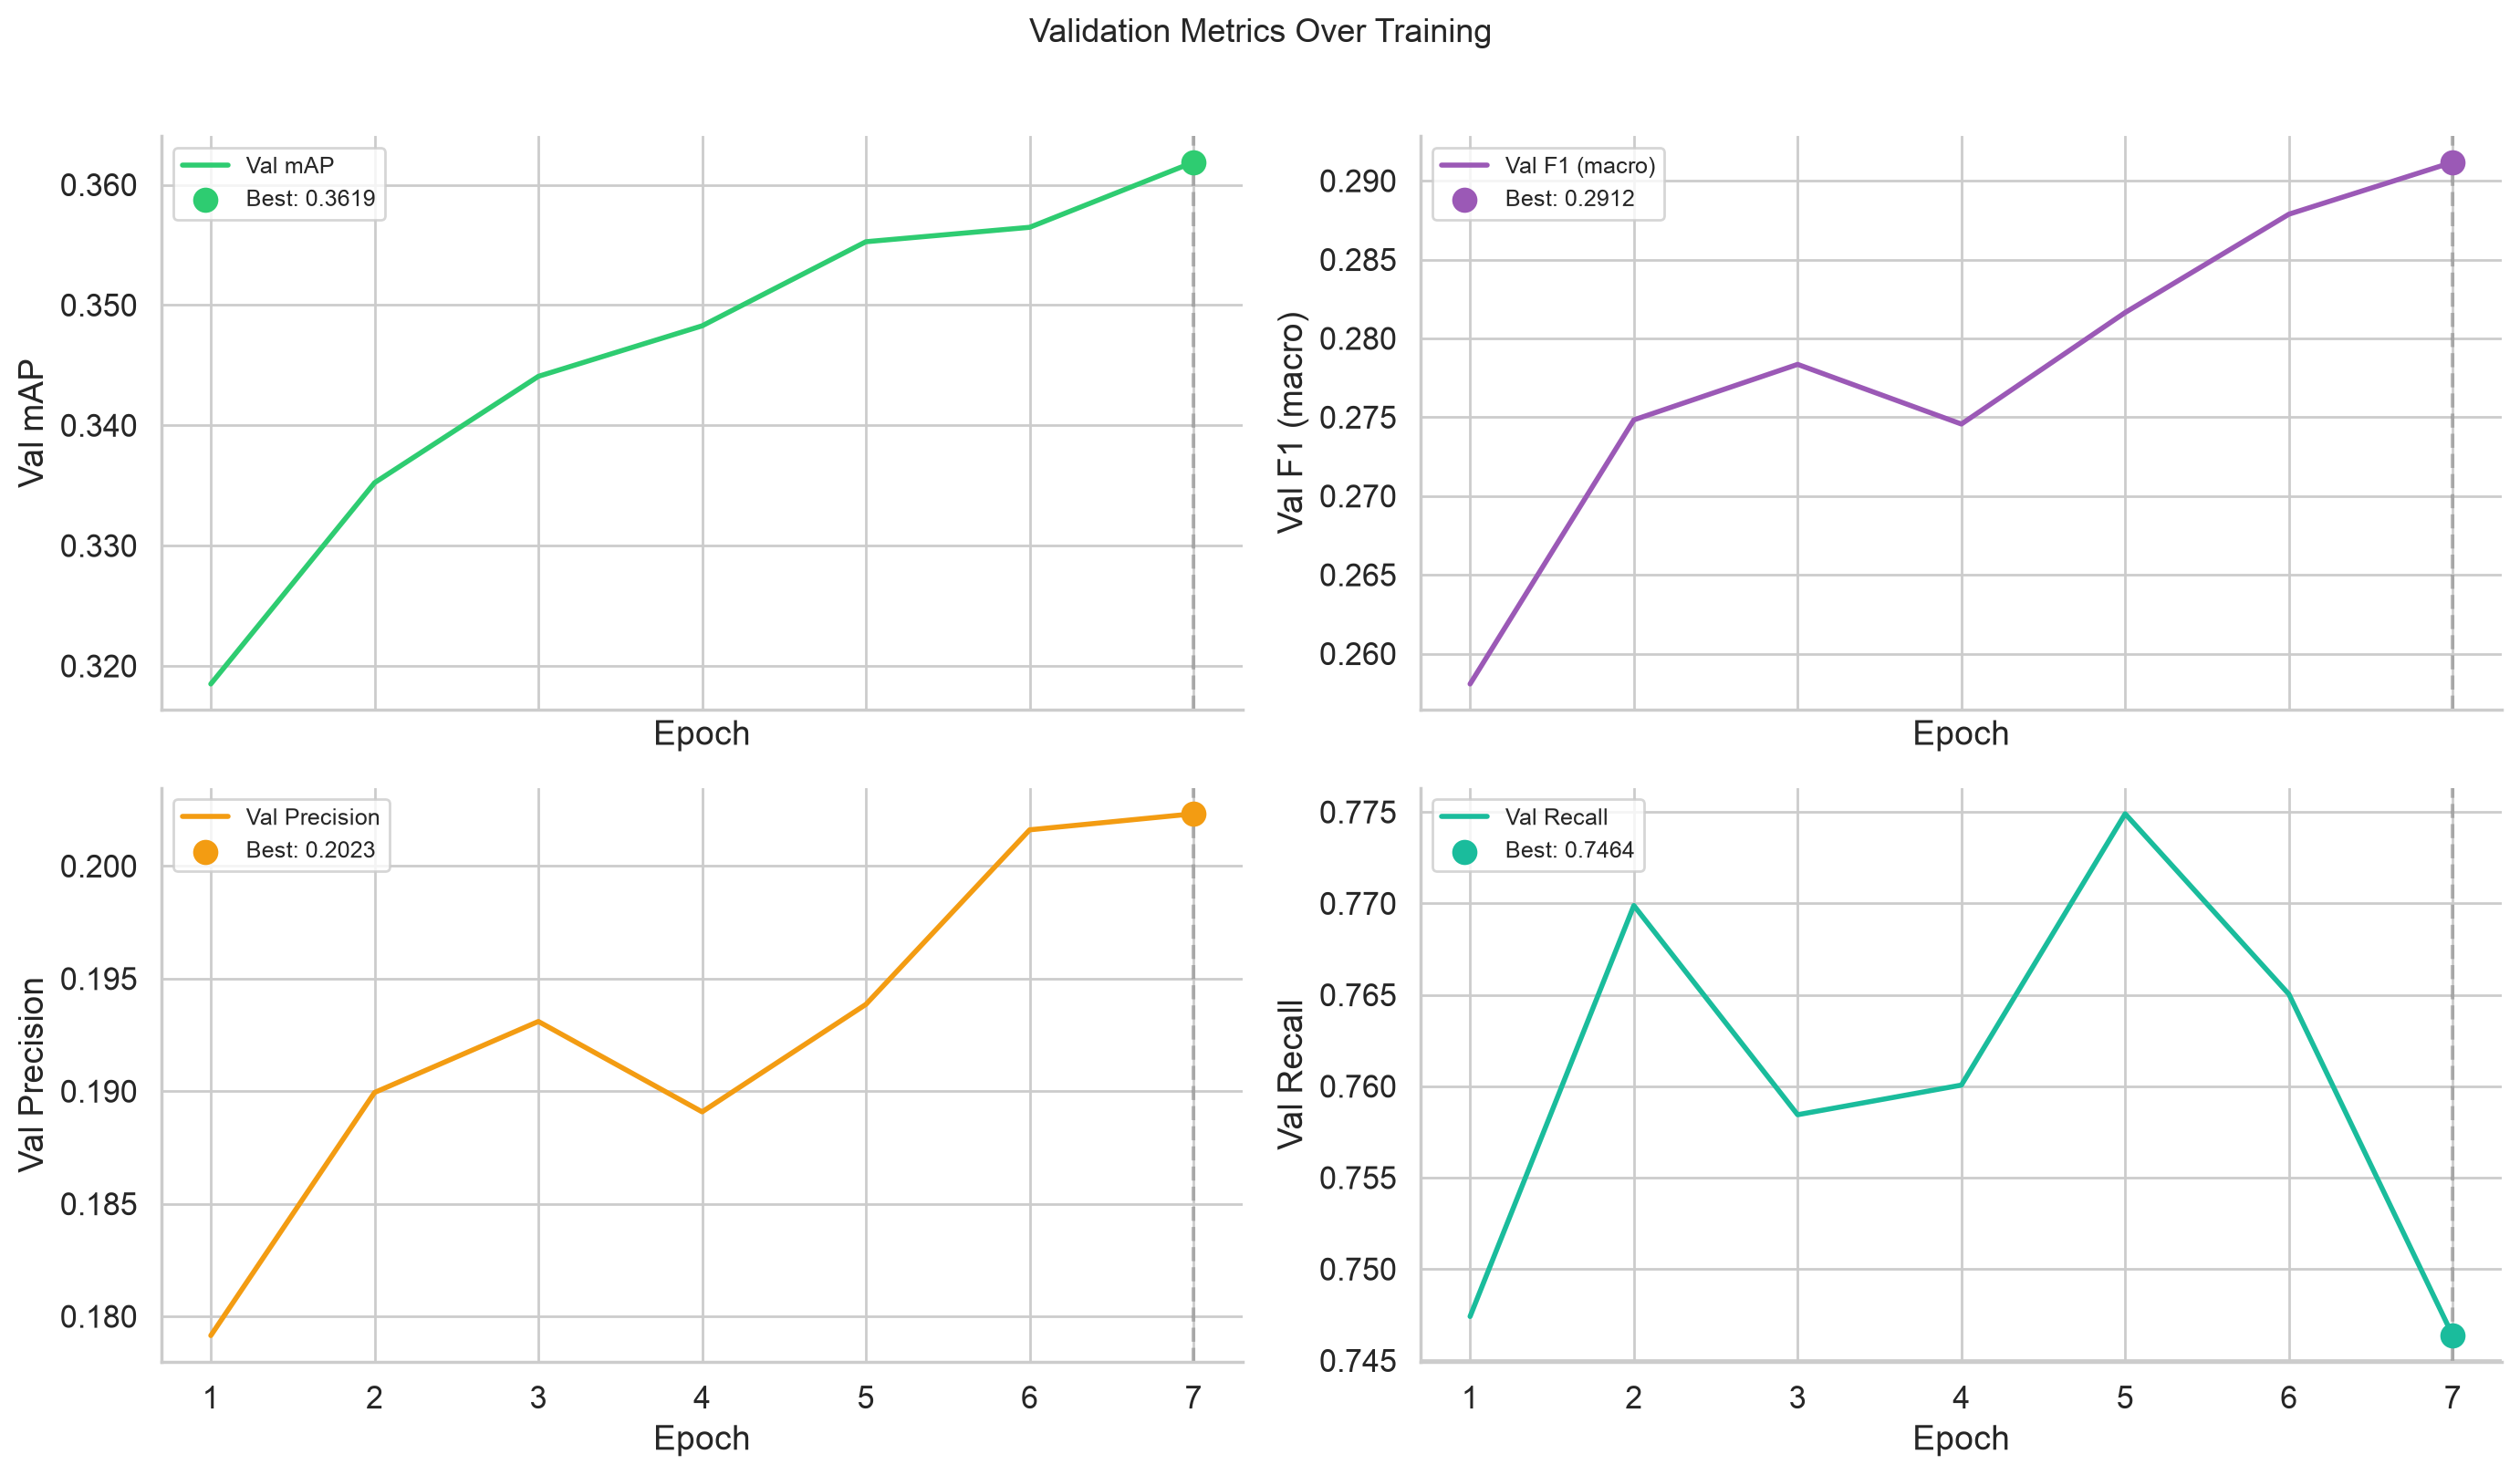
\includegraphics[width=\linewidth]{metric_curves.png}
\caption{Validation mAP, macro-F1, macro-Precision, and macro-Recall across the 7 completed epochs. mAP and F1 climb monotonically; Precision is low and rising slowly; Recall is high (0.75--0.78) and roughly flat.}
\label{fig:metric-curves}
\end{figure}

\begin{figure}[h]
\centering
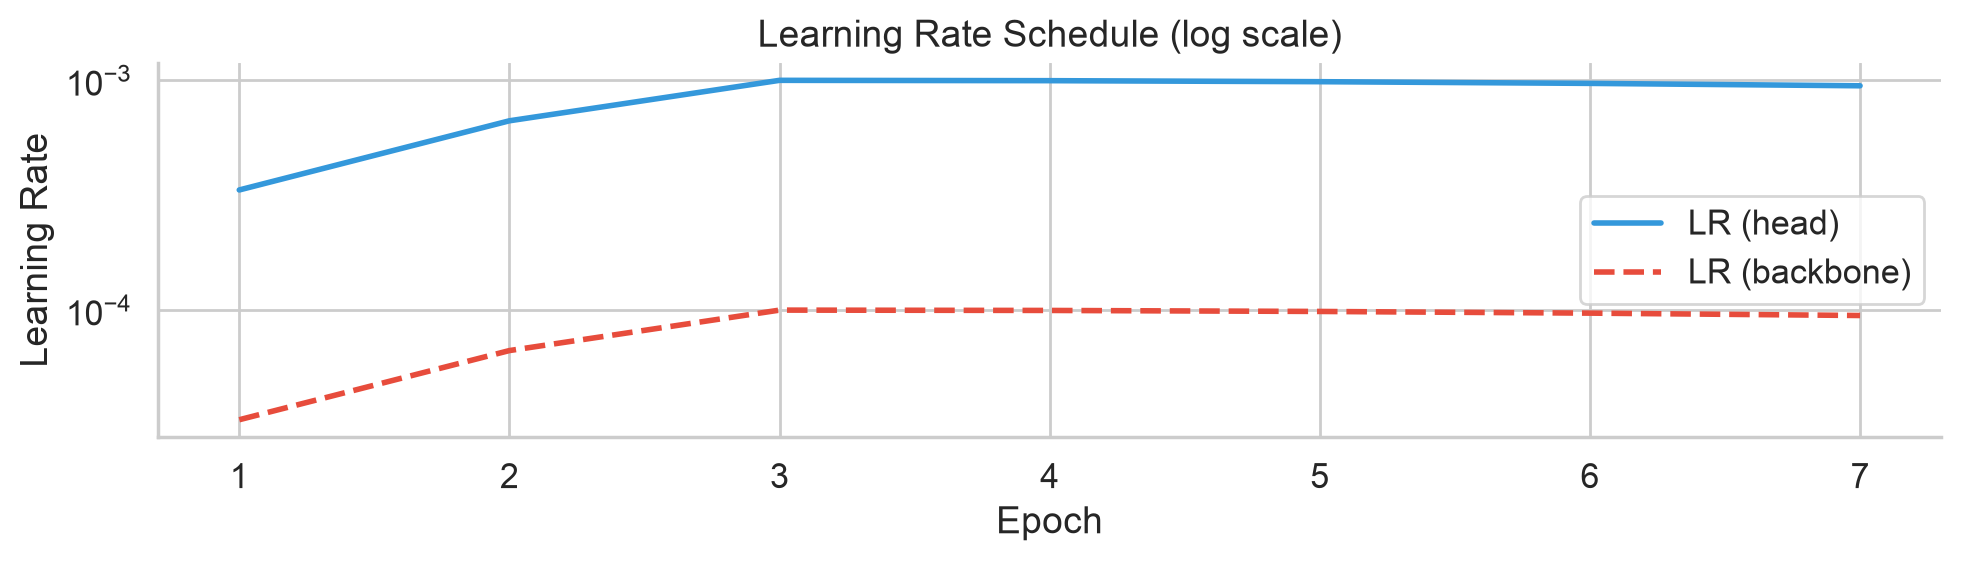
\includegraphics[width=0.85\linewidth]{lr_schedule.png}
\caption{Realized learning-rate schedule for the completed epochs: 3-epoch linear warmup to $\text{lr}_{\text{head}}{=}10^{-3}$ / $\text{lr}_{\text{backbone}}{=}10^{-4}$, followed by the start of cosine decay.}
\label{fig:lr-schedule}
\end{figure}

\subsection{Discussion}

Three things stand out from this early snapshot:

\begin{enumerate}
\item \textbf{Precision/Recall are heavily skewed by \code{pos\_weight}.} At the default 0.5 threshold, macro Recall ($\approx$0.75) is roughly $3.7\times$ macro Precision ($\approx$0.20). Capping \code{pos\_weight} at 50 (median class imbalance is 92.5, so more than half of classes are still capped) trades many false positives for fewer false negatives on rare attributes --- expected behavior, but it means the model as checkpointed is tuned toward over-prediction, and a threshold sweep well above 0.5 (or per-class thresholds) is needed before this checkpoint is production-ready.
\item \textbf{Validation loss already shows an overfitting signal by epoch 5}, even though ranking-based mAP keeps improving. This is a known BCE-with-heavy-\code{pos\_weight} pattern: the loss is dominated by confident wrong predictions on rare positive classes, which can rise even as the model's overall ranking of positives vs.\ negatives (mAP) keeps getting better. It is a reason to prefer mAP (the metric actually used for checkpoint selection) over raw val loss when monitoring this run.
\item \textbf{No epoch count is long enough to compare Ablation A/B/C.} Since A and C were never run, the claim in the config comments that B is the "good balance" configuration is a design hypothesis, not yet an empirically validated result in this repository.
\end{enumerate}

% =====================================================================
\section{Inference Serving Architecture}
% =====================================================================

The trained checkpoint is served behind a FastAPI application (\code{main.py}, \code{app/models.py}) as a three-stage synchronous-per-request pipeline, with all models loaded once at process startup (\code{PipelineManager.load()}) and reused across requests.

\begin{figure}[h]
\centering
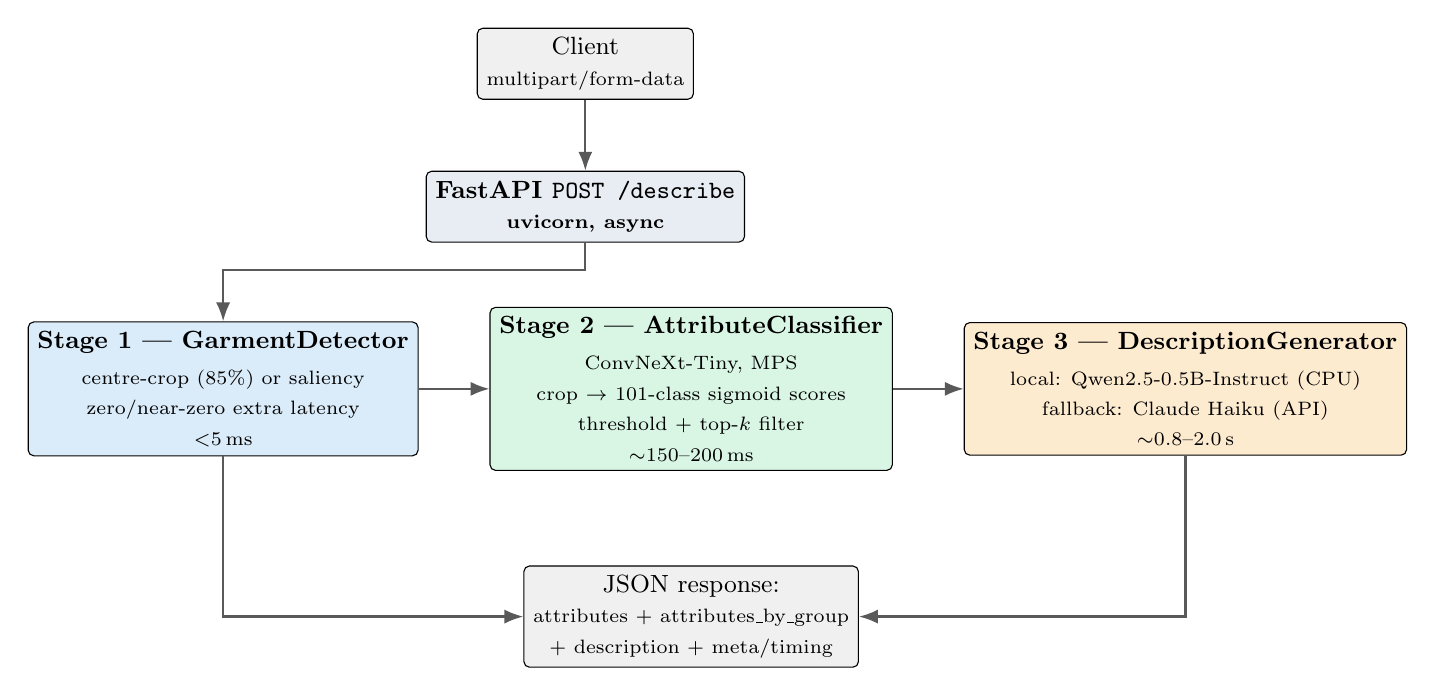
\begin{tikzpicture}[
  ext/.style={draw, rounded corners=2pt, fill=gray!12, minimum height=0.9cm, minimum width=2.6cm, align=center, font=\small},
  api/.style={draw, rounded corners=2pt, fill=cobalt!10, minimum height=0.9cm, minimum width=3.6cm, align=center, font=\small\bfseries},
  s1/.style={draw, rounded corners=2pt, fill=accent2!18, minimum height=1.5cm, minimum width=3.5cm, align=center, font=\small},
  s2/.style={draw, rounded corners=2pt, fill=accent1!18, minimum height=1.5cm, minimum width=3.5cm, align=center, font=\small},
  s3/.style={draw, rounded corners=2pt, fill=accent5!20, minimum height=1.5cm, minimum width=3.5cm, align=center, font=\small},
  arr/.style={-{Latex[length=2.4mm]}, thick, gray!70!black},
  node distance=0.9cm
]
\node[ext] (client) {Client\\ \scriptsize multipart/form-data};
\node[api, below=of client] (fastapi) {FastAPI \code{POST /describe}\\ \scriptsize uvicorn, async};

\node[s1, below=1.0cm of fastapi, xshift=-4.6cm] (stage1) {
  \textbf{Stage 1 --- GarmentDetector}\\[2pt]
  \scriptsize centre-crop (85\%) or saliency\\
  \scriptsize zero/near-zero extra latency\\
  \scriptsize $<$5\,ms
};
\node[s2, right=0.9cm of stage1] (stage2) {
  \textbf{Stage 2 --- AttributeClassifier}\\[2pt]
  \scriptsize ConvNeXt-Tiny, MPS\\
  \scriptsize crop $\to$ 101-class sigmoid scores\\
  \scriptsize threshold + top-$k$ filter\\
  \scriptsize $\sim$150--200\,ms
};
\node[s3, right=0.9cm of stage2] (stage3) {
  \textbf{Stage 3 --- DescriptionGenerator}\\[2pt]
  \scriptsize local: Qwen2.5-0.5B-Instruct (CPU)\\
  \scriptsize fallback: Claude Haiku (API)\\
  \scriptsize $\sim$0.8--2.0\,s
};

\draw[arr] (client) -- (fastapi);
\draw[arr] (fastapi.south) -- ++(0,-0.35) -| (stage1.north);
\draw[arr] (stage1) -- (stage2);
\draw[arr] (stage2) -- (stage3);

\node[ext, below=1.2cm of stage2] (resp) {JSON response:\\ \scriptsize attributes + attributes\_by\_group\\ \scriptsize + description + meta/timing};
\draw[arr] (stage3.south) |- (resp.east);
\draw[arr] (stage1.south) |- (resp.west);
\end{tikzpicture}
\caption{Three-stage inference pipeline behind the \code{/describe} endpoint, orchestrated by \code{PipelineManager}.}
\label{fig:inference-pipeline}
\end{figure}

\subsection{Stage details}

\textbf{Stage 1 --- Garment detection.} The default strategy is a plain \textbf{center crop} (85\% of the frame) rather than an object detector: e-commerce product photos are composited with the garment already filling most of the frame, so a heavy detector (YOLO/Faster-RCNN) would add 200--500\,ms for negligible accuracy gain. A \code{saliency} strategy (classifier-derived activation map) is available in configuration for non-standard, lifestyle-style photos.

\textbf{Stage 2 --- Attribute classification.} The architecture is rebuilt explicitly at load time (rather than unpickling the training class) so the checkpoint stays forward-compatible with code changes; weights are loaded with \code{weights\_only=True} for safety. Predictions above \code{attribute\_threshold} (default \textbf{0.45}) are kept, sorted by confidence, and capped to \code{top\_k\_attributes} (default \textbf{20}); if nothing clears the threshold, the pipeline automatically retries once at threshold 0.3.

\textbf{Stage 3 --- Description generation.} Detected attributes are grouped by supercategory and formatted into a structured prompt (e.g.\ \textit{``Length: midi length (0.87) ... Pattern: floral (0.81) ...''}), then passed to an instruction-tuned LLM with a fixed system prompt asking for a 2--3 sentence product description that does not invent unlisted attributes. Two backends are supported and swappable via \code{.env} with no code change:

\begin{center}
\begin{tabular}{lll}
\toprule
\textbf{Backend} & \textbf{Model} & \textbf{Notes} \\
\midrule
\code{local} (default) & Qwen2.5-0.5B-Instruct & CPU, Apache-2.0, $\sim$1\,GB RAM, $\sim$1.2--2.0\,s \\
\code{claude} & Claude Haiku (Anthropic API) & network call, faster end-to-end ($\sim$0.8--1.2\,s) \\
\bottomrule
\end{tabular}
\end{center}

The local LLM deliberately runs on \textbf{CPU, not MPS} --- ConvNeXt already occupies the MPS device for Stage 2, and HuggingFace \code{generate()} on MPS had known KV-cache issues in some PyTorch versions at the time this was built.

\subsection{Latency budget}

\begin{table}[h]
\centering
\begin{tabular}{lr}
\toprule
\textbf{Stage} & \textbf{Time (M5 MacBook Pro)} \\
\midrule
Image decode + crop & $\sim$5\,ms \\
ConvNeXt-Tiny (MPS) & $\sim$150--200\,ms \\
Qwen2.5-0.5B (CPU) & $\sim$1.2--2.0\,s \\
\midrule
\textbf{Total (local LLM)} & \textbf{$\sim$1.5--2.2\,s} \\
Total (Claude Haiku backend) & $\sim$0.9--1.2\,s (network-dependent) \\
\bottomrule
\end{tabular}
\caption{Expected end-to-end latency, from README benchmarking on an M5 MacBook Pro.}
\end{table}

\subsection{API contract}

\begin{center}
\small
\begin{tabular}{p{3.6cm}p{10.5cm}}
\toprule
\textbf{Endpoint} & \textbf{Behavior} \\
\midrule
\code{POST /describe} & multipart image upload (JPEG/PNG/WEBP, max 15\,MB) $\to$ attributes + grouped attributes + description + inference metadata (crop box, thresholds, model IDs, per-stage timing) \\
\code{GET /health} & liveness/readiness probe reporting model-loaded status, backend, and device \\
\bottomrule
\end{tabular}
\end{center}

% =====================================================================
\section{Key Engineering Decisions --- Summary}
% =====================================================================

\begin{itemize}
\item \textbf{Crop-level training, not image-level}, because Fashionpedia attributes are properties of garment parts, not whole photos.
\item \textbf{Drop rather than negate} zero-attribute annotations, to avoid injecting false negatives from annotator skips.
\item \textbf{Exclude \emph{nickname}} attributes from the visual-attribute head; they are category identifiers, not visual descriptors, and would need a separate head if modeled at all.
\item \textbf{Partial fine-tuning with differential LR} instead of full fine-tuning or head-only training, to balance adaptation speed against catastrophic forgetting of ImageNet features, with an explicit ablation axis (\code{unfreeze\_from\_block}) to make that trade-off tunable.
\item \textbf{\code{pos\_weight}-weighted BCE, capped at 50}, to make the 101-class label space (imbalance up to 515$\times$) learnable without exploding gradients on the rarest classes.
\item \textbf{Center-crop over a learned detector} for garment localization, favoring the empirical structure of e-commerce photography over general-purpose object detection.
\item \textbf{A small local LLM with an API fallback} for description generation, trading a slightly higher local latency for zero per-request cost and no external dependency, while keeping a faster network-backed option available.
\end{itemize}

% =====================================================================
\section{Limitations and Future Work}
% =====================================================================

\begin{itemize}
\item \textbf{The reported model is an early checkpoint (epoch 7/30), not a converged one.} \code{val\_mAP} was still climbing when logging stopped; a full 30-epoch (or longer, with LR re-tuned) run is needed before drawing firm conclusions about Ablation-B's ceiling.
\item \textbf{Ablations A and C were never executed}, so the claim that "stage-4 + head" is the right amount of fine-tuning is currently a design hypothesis rather than an empirical result.
\item \textbf{No final threshold sweep exists for the real model.} Given the precision/recall imbalance already visible by epoch 7, retuning \code{attribute\_threshold} (currently 0.45 in serving, vs.\ 0.5 in the training-time metric) or moving to per-class thresholds is a likely next step.
\item \textbf{The category$\leftrightarrow$attribute affinity table is not being used}, and the exported heatmap artifact currently reads all zeros --- worth revisiting if category-conditioned masking is pursued.
\item \textbf{The center-crop detector is a strong assumption} about photo composition; it will underperform on lifestyle/editorial photography where the garment does not fill the frame, which is what the (currently stubbed-out) saliency strategy is meant to address.
\item \textbf{No offline evaluation of the generated descriptions exists} (e.g.\ faithfulness to detected attributes, fluency); Stage 3 is currently validated only by manual inspection of example outputs.
\end{itemize}

% =====================================================================
\section{Conclusion}
% =====================================================================

This project implements a complete, working pipeline from raw Fashionpedia annotations to a served product-description API: a carefully justified preprocessing pipeline that turns noisy multi-label garment-part annotations into a clean 101-class dataset; a ConvNeXt-Tiny classifier trained with partial fine-tuning, differential learning rates, and imbalance-aware loss; and a three-stage FastAPI inference service that composes the classifier with a local or API-backed LLM for natural-language product copy. The infrastructure --- ablation configs, training-curve tooling, structured logging --- is in place for a rigorous comparison of fine-tuning strategies; what remains is running the experiments to completion. The single training run captured in this repository (Ablation B, 7 of 30 epochs) already reaches a validation mAP of 0.362 and macro-F1 of 0.291 while still improving, suggesting meaningful headroom is left on the table by the interrupted run.

\end{document}
